% Options for packages loaded elsewhere
\PassOptionsToPackage{unicode}{hyperref}
\PassOptionsToPackage{hyphens}{url}
\PassOptionsToPackage{dvipsnames,svgnames,x11names}{xcolor}
%
\documentclass[
]{agujournal2019}

\usepackage{amsmath,amssymb}
\usepackage{iftex}
\ifPDFTeX
  \usepackage[T1]{fontenc}
  \usepackage[utf8]{inputenc}
  \usepackage{textcomp} % provide euro and other symbols
\else % if luatex or xetex
  \usepackage{unicode-math}
  \defaultfontfeatures{Scale=MatchLowercase}
  \defaultfontfeatures[\rmfamily]{Ligatures=TeX,Scale=1}
\fi
\usepackage{lmodern}
\ifPDFTeX\else  
    % xetex/luatex font selection
\fi
% Use upquote if available, for straight quotes in verbatim environments
\IfFileExists{upquote.sty}{\usepackage{upquote}}{}
\IfFileExists{microtype.sty}{% use microtype if available
  \usepackage[]{microtype}
  \UseMicrotypeSet[protrusion]{basicmath} % disable protrusion for tt fonts
}{}
\makeatletter
\@ifundefined{KOMAClassName}{% if non-KOMA class
  \IfFileExists{parskip.sty}{%
    \usepackage{parskip}
  }{% else
    \setlength{\parindent}{0pt}
    \setlength{\parskip}{6pt plus 2pt minus 1pt}}
}{% if KOMA class
  \KOMAoptions{parskip=half}}
\makeatother
\usepackage{xcolor}
\setlength{\emergencystretch}{3em} % prevent overfull lines
\setcounter{secnumdepth}{5}
% Make \paragraph and \subparagraph free-standing
\makeatletter
\ifx\paragraph\undefined\else
  \let\oldparagraph\paragraph
  \renewcommand{\paragraph}{
    \@ifstar
      \xxxParagraphStar
      \xxxParagraphNoStar
  }
  \newcommand{\xxxParagraphStar}[1]{\oldparagraph*{#1}\mbox{}}
  \newcommand{\xxxParagraphNoStar}[1]{\oldparagraph{#1}\mbox{}}
\fi
\ifx\subparagraph\undefined\else
  \let\oldsubparagraph\subparagraph
  \renewcommand{\subparagraph}{
    \@ifstar
      \xxxSubParagraphStar
      \xxxSubParagraphNoStar
  }
  \newcommand{\xxxSubParagraphStar}[1]{\oldsubparagraph*{#1}\mbox{}}
  \newcommand{\xxxSubParagraphNoStar}[1]{\oldsubparagraph{#1}\mbox{}}
\fi
\makeatother


\providecommand{\tightlist}{%
  \setlength{\itemsep}{0pt}\setlength{\parskip}{0pt}}\usepackage{longtable,booktabs,array}
\usepackage{calc} % for calculating minipage widths
% Correct order of tables after \paragraph or \subparagraph
\usepackage{etoolbox}
\makeatletter
\patchcmd\longtable{\par}{\if@noskipsec\mbox{}\fi\par}{}{}
\makeatother
% Allow footnotes in longtable head/foot
\IfFileExists{footnotehyper.sty}{\usepackage{footnotehyper}}{\usepackage{footnote}}
\makesavenoteenv{longtable}
\usepackage{graphicx}
\makeatletter
\newsavebox\pandoc@box
\newcommand*\pandocbounded[1]{% scales image to fit in text height/width
  \sbox\pandoc@box{#1}%
  \Gscale@div\@tempa{\textheight}{\dimexpr\ht\pandoc@box+\dp\pandoc@box\relax}%
  \Gscale@div\@tempb{\linewidth}{\wd\pandoc@box}%
  \ifdim\@tempb\p@<\@tempa\p@\let\@tempa\@tempb\fi% select the smaller of both
  \ifdim\@tempa\p@<\p@\scalebox{\@tempa}{\usebox\pandoc@box}%
  \else\usebox{\pandoc@box}%
  \fi%
}
% Set default figure placement to htbp
\def\fps@figure{htbp}
\makeatother
% definitions for citeproc citations
\NewDocumentCommand\citeproctext{}{}
\NewDocumentCommand\citeproc{mm}{%
  \begingroup\def\citeproctext{#2}\cite{#1}\endgroup}
\makeatletter
 % allow citations to break across lines
 \let\@cite@ofmt\@firstofone
 % avoid brackets around text for \cite:
 \def\@biblabel#1{}
 \def\@cite#1#2{{#1\if@tempswa , #2\fi}}
\makeatother
\newlength{\cslhangindent}
\setlength{\cslhangindent}{1.5em}
\newlength{\csllabelwidth}
\setlength{\csllabelwidth}{3em}
\newenvironment{CSLReferences}[2] % #1 hanging-indent, #2 entry-spacing
 {\begin{list}{}{%
  \setlength{\itemindent}{0pt}
  \setlength{\leftmargin}{0pt}
  \setlength{\parsep}{0pt}
  % turn on hanging indent if param 1 is 1
  \ifodd #1
   \setlength{\leftmargin}{\cslhangindent}
   \setlength{\itemindent}{-1\cslhangindent}
  \fi
  % set entry spacing
  \setlength{\itemsep}{#2\baselineskip}}}
 {\end{list}}
\usepackage{calc}
\newcommand{\CSLBlock}[1]{\hfill\break\parbox[t]{\linewidth}{\strut\ignorespaces#1\strut}}
\newcommand{\CSLLeftMargin}[1]{\parbox[t]{\csllabelwidth}{\strut#1\strut}}
\newcommand{\CSLRightInline}[1]{\parbox[t]{\linewidth - \csllabelwidth}{\strut#1\strut}}
\newcommand{\CSLIndent}[1]{\hspace{\cslhangindent}#1}

\usepackage{url} %this package should fix any errors with URLs in refs.
\usepackage{lineno}
\usepackage[inline]{trackchanges} %for better track changes. finalnew option will compile document with changes incorporated.
\usepackage{soul}
\linenumbers
\makeatletter
\@ifpackageloaded{caption}{}{\usepackage{caption}}
\AtBeginDocument{%
\ifdefined\contentsname
  \renewcommand*\contentsname{Table of contents}
\else
  \newcommand\contentsname{Table of contents}
\fi
\ifdefined\listfigurename
  \renewcommand*\listfigurename{List of Figures}
\else
  \newcommand\listfigurename{List of Figures}
\fi
\ifdefined\listtablename
  \renewcommand*\listtablename{List of Tables}
\else
  \newcommand\listtablename{List of Tables}
\fi
\ifdefined\figurename
  \renewcommand*\figurename{Figure}
\else
  \newcommand\figurename{Figure}
\fi
\ifdefined\tablename
  \renewcommand*\tablename{Table}
\else
  \newcommand\tablename{Table}
\fi
}
\@ifpackageloaded{float}{}{\usepackage{float}}
\floatstyle{ruled}
\@ifundefined{c@chapter}{\newfloat{codelisting}{h}{lop}}{\newfloat{codelisting}{h}{lop}[chapter]}
\floatname{codelisting}{Listing}
\newcommand*\listoflistings{\listof{codelisting}{List of Listings}}
\makeatother
\makeatletter
\makeatother
\makeatletter
\@ifpackageloaded{caption}{}{\usepackage{caption}}
\@ifpackageloaded{subcaption}{}{\usepackage{subcaption}}
\makeatother
\makeatletter
\@ifpackageloaded{sidenotes}{}{\usepackage{sidenotes}}
\@ifpackageloaded{marginnote}{}{\usepackage{marginnote}}
\makeatother

\usepackage{bookmark}

\IfFileExists{xurl.sty}{\usepackage{xurl}}{} % add URL line breaks if available
\urlstyle{same} % disable monospaced font for URLs
\hypersetup{
  pdftitle={Distinct functional responses of consumers and their producers to climate drive mutualistic network asymmetry},
  pdfauthor={Gabriel Munoz; Paul Savary; W. Daniel Kissling; JP Lessard},
  pdfkeywords={Climate change, Frugivory, Interaction diversity, Network
specialization, Seed dispersal},
  colorlinks=true,
  linkcolor={blue},
  filecolor={Maroon},
  citecolor={Blue},
  urlcolor={Blue},
  pdfcreator={LaTeX via pandoc}}



\draftfalse

\begin{document}
\title{Distinct functional responses of consumers and their producers to
climate drive mutualistic network asymmetry}

\authors{Gabriel Munoz\affil{1}, Paul Savary\affil{1}, W. Daniel
Kissling\affil{2}, JP Lessard\affil{1}}
\affiliation{1}{Concordia University, }\affiliation{2}{University of
Amsterdam, }
\correspondingauthor{Gabriel Munoz}{gabrielmunoz1891@gmail.com}


\begin{abstract}
\textbf{Aim:} Functional traits are often used to infer the ecological
processes that determine the composition of species assemblages. Whereas
most trait-based approaches to infer community assembly processes focus
on a single trophic level, traits also mediate interactions between
trophic levels. Owing to the matching of traits facilitating
interactions between resource and consumer assemblages, the functional
trait diversity of different trophic levels is expected to covary in
space. However, the differential response of consumers and producers to
environmental gradients can cause a decoupling of functional diversity
between trophic levels, which we coin functional trophic asymmetry.
Here, we develop a metric to quantify functional trophic asymmetry (FTA)
and use it to infer the processes underpinning multitrophic community
assembly and explore the role of these processes in shaping the topology
of ecological networks.

\textbf{Location:} Neotropics.

\textbf{Time period:} Present.

\textbf{Major taxa:} Mammalian frugivores and palms.

\textbf{Methods:} We used digitally available data on the functional
traits, pairwise mutualistic interactions, and geographic distributions
of consumers (mammalian frugivores) and their producers (palms) to
quantify FTA for species assemblages occurring in the Neotropics. To
cover major data gaps between species-level trait and interaction data
at finer spatial grain, we trained machine learning models to downscale
the continental meta-network to grid cell-level networks. For each
grid-cell, we also estimated FTA for all combinations of interaction
guilds. These guilds were defined as distinct subsets of producer and
consumer assemblages playing similar roles within mutualistic networks
and sharing partners in the other trophic level. We then use generalized
additive models to relate geographic variation in FTA to variation in
climatic variables and assessed whether the strength of these
relationship varied among pairwise interaction guilds. Finally, we then
examined the relationship between FTA and network specialization.

\textbf{Results:} By downscaling the continental metaweb, we generated
probabilistic networks across 1,072 grid cells in the Neotropics. Our
modelling approach identified 7 consumer and 7 producer interaction
guilds. Assemblage-wide FTA is negatively related to annual mean
temperatures across the neotropics. When considering individual
interaction guilds, precipitation seasonality is positively related to
FTA. This relationship between FTA and precipitation seasonality was
stronger for consumer and producer guild combinations with high
predicted interaction strength. Finally, network specialization was
positively related to FTA, regardless of the interaction guild
combination.

\textbf{Main conclusions:} Mutualistic networks in warm regions with
seasonal rainfalls, where the environment imposes a disproportionately
strong selective pressure on palms relative to mammal frugivores,
exhibit higher levels of functional trophic asymmetry. This relationship
is particularly strong when considering guilds predicted to strongly
interact in nature. Assemblages exhibiting high FTA also tend to have
high levels of network specialization, suggesting that differences in
the strength of environmental selection among trophic levels favor the
persistence of specialist species in these mutualistic interaction
networks. We therefore conclude that future increases in temperature and
the magnitude of precipitation seasonality caused by global climate
change could lead to more specialized mutualistic networks which are
more prone to collapse when facing further threats and local
extinctions.
\end{abstract}





\section{Introduction}\label{introduction}

Ecologists often examine patterns of functional trait diversity to
investigate community assembly processes (Ackerly, 2003; Kraft et al.,
2015). To date, however, trait-based approaches in ecology often focus
on a single trophic level, whereas approaches that consider multiple
trophic levels remain rare (Lavorel et al., 2013; Seibold et al., 2018).
An approach that considers processes operating within and between
trophic levels is necessary to better understand the assembly of
multitrophic communities(Allesina et al., 2008; Marjakangas et al.,
2022; Saravia et al., 2022). Moreover, considering trophic interactions
while studying community assembly could shed new light on processes
underpinning ecological networks (Allesina et al., 2008) .

Classical approaches to study community assembly rely on the concept of
environmental filtering, sorting or selection, where density independent
conditions constrain the functional richness of species assemblages
(HilleRisLambers et al., 2012; Kraft et al., 2015; Laliberté \&
Legendre, 2010; Villéger et al., 2008). Functional richness refers to
the variability and relative frequency of different functional traits
observed in a community. It is often used to estimate the strength of
selection imposed by the environment (Kraft et al., 2008, 2015; Kraft \&
Ackerly, 2010). High functional richness can indicate weak environmental
selection whereas low functional richness can indicate strong selection
(Halpern \& Floeter, 2008; Kraft et al., 2008; Paine et al., 2011). In a
multitrophic context, the effects of environmental selection can cascade
across trophic levels such that selection on consumer traits can shape
the functional richness of their resources, modulated by their degree of
reciprocal dependency or co-evolution (Guzman et al., 2019; Lavorel et
al., 2013). Moreover, the same environmental gradient could exert
selective pressures of different strength on communities at distinct
trophic levels (Marjakangas et al., 2022). Differences in the strength
of selective pressure among trophic levels could then possibly constrain
the structure or topologies of trophic networks (Blüthgen et al., 2007;
Dehling et al., 2020; Schleuning et al., 2012).

Inferring the relative strength of environmental selection between
trophic levels requires using high-dimensional approaches that are able
to deal with sparse observations for a large number of species (Rohr et
al., 2010; Strydom et al., 2022). We introduce the concept of functional
trophic asymmetry (FTA), which allows inferring the relative influence
of environmental selection and trait matching on the composition of
multitrophic assemblages \href{Figure\%201}{(Figure 1)}. FTA is the
difference in the richness of interaction-relevant traits between
trophic levels in a multitrophic network. FTA can occur because traits
mediating species interactions (i.e., interaction niches) across trophic
levels can also mediate the responses of species to their abiotic
environment (i.e.~environmental niches) (Dehling et al., 2020; McCain \&
King, 2014; Moretti \& Legg, 2009; Nagy et al., 2018). As an example,
plant seed size determine the outcome of animal-mediated seed dispersal
(Donoso et al., 2017, 2020) as well as physiological limits, such as
tolerances of plant seedlings to desiccation (Hoekstra et al., 2001).
High FTA could indicate differences in the strength of environmental
selection over the interaction niches of distinct trophic levels within
a multitrophic species assemblage. Alternatively, low FTA could indicate
that the strength of the environment selection shaping interaction
niches is similar between trophic levels, e.g.~equally weak or equally
strong (Marjakangas et al., 2022). When interactions between producers
and consumers are mutualistic, low FTA could also emerge under strong
trait matching and therefore indicate the influence of trait-coevolution
during multitrophic community assembly (Albrecht et al., 2018; Dehling
et al., 2014). By studying spatial variation in functional trophic
asymmetry along environmental gradients, we could possibly identify the
conditions promoting environmentally versus cross-trophic interaction-
driven community assembly (Bello et al., 2023; Schleuning et al., 2020).

Frameworks linking multitrophic functional diversity to network topology
along broad-scale environmental gradients are crucial to understand the
effects of global change on biodiversity and ecosystem function (Bello
et al., 2023; Dehling, 2018; Schleuning et al., 2014, 2020, 2023).
Functional responses of consumer and producer assemblages to climate
influence functional richness at the level of the multitrophic community
(Garcı́a et al., 2018). Because some of these traits are involved in
interactions across trophic levels, the filtering of traits along
environmental gradients could constrain the number of unique
interactions and therefore, network topology (Albrecht et al., 2018;
Emer et al., 2020; Marjakangas et al., 2022). As an example, low
multitrophic functional richness could influence emergent patterns in
network structure such as the specialization of multispecies
interactions by limiting the relative availability of interaction
partners across trophic levels (Blüthgen et al., 2006, 2007). While high
levels of network specialization represent networks predominantly made
of ``one-to-one'' interactions, low levels of network specialization
represent networks with species showing predominantly ``one-to-many''
interactions (Blüthgen et al., 2006; Blüthgen \& Klein, 2011) (Figure
1B). One highly expected outcome is that when functional trophic
asymmetry is high, networks will have low specialization. For example,
take a plant community exhibiting a low richness of flower displays and
which is associated with a bee community (pollinators) exhibiting a wide
variety of proboscis lengths. These plants are unlikely to form
``one-to-one'' interactions with only a subset of bee species that have
matching proboscis length. Otherwise, non-matching pollinators would
have no food resource and be extirpated. By partitioning deviations from
expected FTA and network specialization relationships with null models,
one can separate the relative influences of processes operating between
trophic levels (e.g.~trait matching) and those within trophic levels
(e.g.~environmental selection) in network assembly (Marjakangas et al.,
2022). However, the relationship between network specialization and
functional trophic asymmetry has not been fully explored.

Preserving mutualistic interactions between palms and their mammalian
frugivores is important to sustain biodiversity and ecosystem function
in the tropics (Bogoni et al., 2020; Marques Dracxler \& Kissling,
2022). Mammalian frugivores facilitate the dispersal of palm fruits,
which helps to prevent local extinctions amid disturbance and to
maintain biodiversity in these ecological networks (Acevedo-Quintero et
al., 2020; Dehling, 2018; Messeder et al., 2020). To effectively
preserve these interactions, it is crucial to understand how palm
(producer) and frugivore (consumer) communities together respond to
environmental gradients (Pereira et al., 2022). By examining the
co-variation in their functional richness across broad geographic scales
and link those patterns to spatial and/or temporal variation in climate,
we can identify key abiotic factors that influence the assembly of their
mutualistic relationships (Albrecht et al., 2018; Schleuning et al.,
2020). Here, we ask (1) which climatic variable(s) best explains
geographic variation in the functional richness of palms and mammal
frugivores, (2) whether differences in these relationships lead to
functional trophic asymmetry (hereafter FTA), and (3) which climatic
variable best explains geographic variation in FTA across the
Neotropics. We also ask (4) whether the strength of interactions between
palms and mammal frugivores that occupy similar roles in the mutualistic
network relates to the strength of the relationship between FTA and
climate. Finally, we ask (5) whether geographic variation in FTA relates
to network specialization.

\begin{figure}[H]

{\centering \pandocbounded{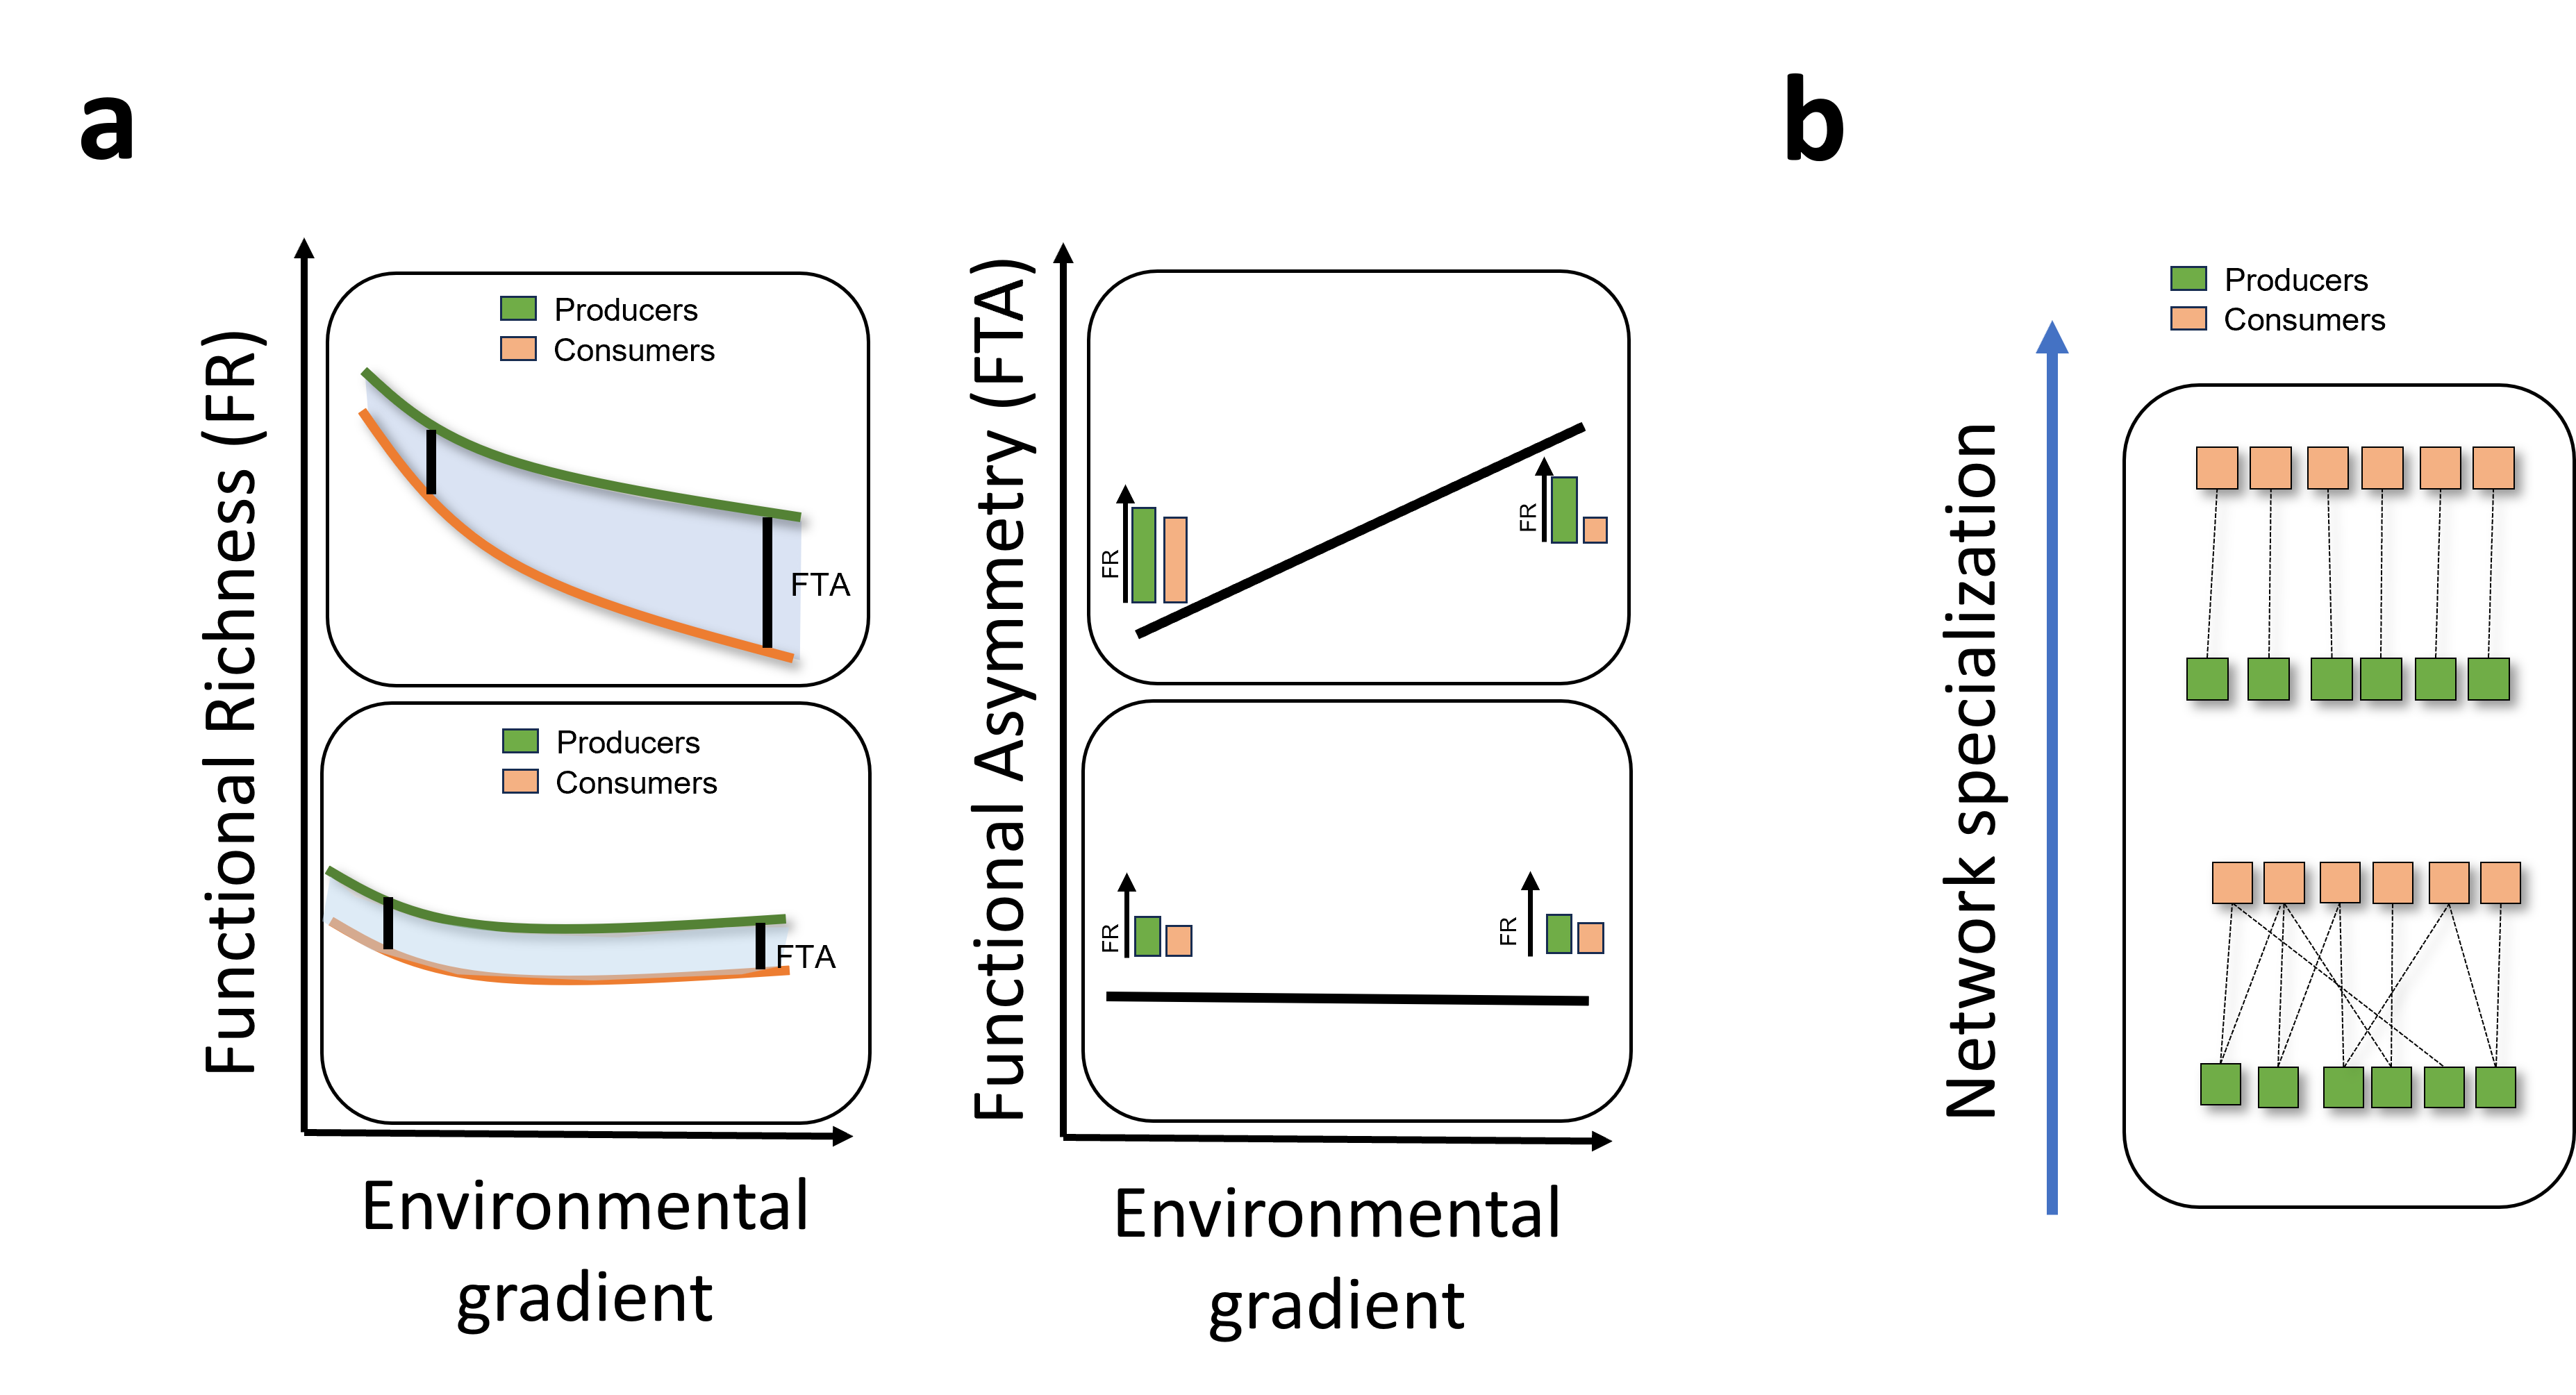
\includegraphics[keepaspectratio]{Main_figures/00_Figure1.png}}

}

\caption{\textbf{Figure 1:} This conceptual model illustrates the
dynamic relationship between functional diversity metrics---specifically
Functional Richness (FR) and Functional Trait Asymmetry (FTA)---and
environmental gradients within ecological networks. The left panel of
\textbf{Figure A} visualizes the variation in FR for producers (depicted
in green) and consumers (depicted in orange) along an environmental
gradient. As the environmental gradient intensifies (e.g., through
changes in temperature, precipitation, or habitat fragmentation), FR for
both producers and consumers generally declines. However, this decline
can occur at different rates, leading to two scenarios: (1)
\textbf{Differential Decline in FR}: If consumer FR declines more
sharply than producer FR, a substantial increase in Functional Trait
Asymmetry (FTA) occurs. (2) \textbf{Parallel Decline in FR}:
Alternatively, if both producer and consumer FRs decline at a similar
rate, FTA remains relatively constant along the gradient. This scenario
indicates a balanced impact of environmental changes across trophic
levels, preserving the relative functional relationship between
producers and consumers. \textbf{Figure B} shifts focus to the
implications of changing FTA on network specialization---a measure of
how distinct or generalized interactions are between producers and
consumers within ecological networks. \textbf{Higher Specialization}:
This scenario, shown on the left side of the gradient, involves more
distinct producer-consumer interactions, where specific consumer species
interact with particular producer species. This high specialization
often correlates with low FTA, where the functional traits between
interacting species are closely aligned. \textbf{Lower Specialization}:
As environmental stress increases, leading to a higher FTA, the network
may shift towards lower specialization. In this state, interactions
become more generalized, with consumers utilizing a broader range of
producers due to the loss of specific functional traits.}

\end{figure}%

\section{Methods}\label{methods}

\subsection{Study system}\label{study-system}

We focused on multitrophic communities of Neotropical palms and their
mutualistic, seed dispersing, mammalian frugivores (Figure S1). Palms
(Plantae:Arecaceae), being a keystone plant family in tropical regions
(Kissling et al.~2012; Onstein et al.~2017), provide fruit resources to
a wide variety of vertebrate frugivores, including birds and mammals
(Muñoz, Trøjelsgaard, and Kissling 2019; Zona and Henderson 1989).
Frugivore mammals (Animalia:Mammalia) are among the most important
palm-seed dispersers, particularly over long distances. Most frugivore
mammals feeding on palms are seed eaters and pulp eaters, dispersing
palm seeds mostly via ectozoochorus dispersal (Messeder et al.~2020).
Importantly, frugivory-related traits have notably underlain palm
diversification and played a key role in the evolution of palm traits
(Onstein et al.~2014, 2017)

\subsubsection{Geographic distribution
data}\label{geographic-distribution-data}

We obtained binary species distribution data (present/absent) on palms
from the geographic range maps of (Bjorholm et al.~2005) and on mammals
from the IUCN (International Union for the Conservation of Nature) data
portal. To generate local gridded multitrophic species assemblages
across the Neotropics, we intersected the species-level range maps with
a spatial grid where each grid cell represented every 1 by 1 degree
latitude and longitude change along the extent of the entire Neotropics.
We then listed all palm and mammal frugivore species co-occurring in
each grid-cell as our grid-cell level multitrophic assemblage.

\subsubsection{Trait data}\label{trait-data}

We collected species-level multitrophic trait data related to the
physiological tolerance of palms and frugivorous mammals to the abiotic
environment and to their mutualistic interactions. For palms, we
extracted data from the PalmTraits 1.0 dataset (Kissling et al.~2019).
We collected data on growth form, maximum stem height, and average fruit
length. For frugivorous mammals, we obtained trait data from the
EltonTraits 1.0 database (Wilman et al.~2014). We selected data on body
mass, diet, and daily activities. Diet data from the EltonTraits 1.0
database is coded as percentage use distribution across ten diet
categories. We excluded from our analysis species without fruit in their
diet. Activity was coded as a dummy variable with three categories
(Diurnal, Crepuscular, Nocturnal). Finally, body mass was coded as a
numerical variable in kg. We excluded bats from the analysis as almost
no Neotropical bat species is feeding on palm fruits (Messeder et al.
2020). In total, we subset from this dataset the species with available
distribution range map, that is 494 palm species and 737 mammal
frugivores.

\subsubsection{Pairwise interaction
data}\label{pairwise-interaction-data}

We used data on seed dispersal interactions between palms and mammals
for the Neotropics, originating from recollections of seed dispersal
records found in the published literature and interaction records are
recorded at the species level (Muñoz, Trøjelsgaard, and Kissling 2019).
Each pairwise species interaction record reflects where an article
mentions the fruit or the seed of a palm being dispersed, carried or
defecated by a frugivorous mammal. Interaction records collected in this
database were previously vetted to reflect effective seed dispersal
interactions, while avoiding those that reflect mere seed consumption
(vetting criteria found in: Muñoz, Trøjelsgaard, and Kissling 2019). In
total, we gathered a total of 581 interaction records between 69 palms
and 111 frugivore mammals.

\subsubsection{Environmental data}\label{environmental-data}

We used bioclimatic variables from WorldClim (Fick and Hijmans 2017) to
represent large-scale spatial and temporal variation of climate in the
Neotropics. Specifically, we used mean annual temperature (BIO01), total
annual precipitation (BIO12), temperature seasonality (BIO04) and
precipitation seasonality (BIO15). Using a moving window, we compute
simple averages for every set of bioclimatic records at each grid cell,
thereby re-scaling the spatial resolution of bioclimatic variables to 1
by 1 degree grid resolution from their original resolution (1 ´ 1
km\textsuperscript{2}) to match the spatial resolution of our grid cell
species-level data.

\subsubsection{Species pool delineation}\label{species-pool-delineation}

The Neotropics is a region with a rich evolutionary history which
significantly influenced patterns of species colonization and extinction
across neotropical plant and animal species (Whiteman-Jennings 2015;
Antonelli and Sanmartı́n 2011).We used the biogeographic regionalization
of Morrone (2014) to delineate the spatial extent of species pools when
simulating network assembly processes. These seven major biogeographic
regions (i.e., biogeographic dominions) were delineated based on
evolutionary history, distributional patterns and ecological
characteristics of both plants and animals in the Neotropics. ~

\subsection{\texorpdfstring{\textbf{Statistical
analyses}}{Statistical analyses}}\label{statistical-analyses}

\subsubsection{\texorpdfstring{\emph{Building a probabilistic
continental metaweb from aggregated binary interaction
records}}{Building a probabilistic continental metaweb from aggregated binary interaction records}}\label{building-a-probabilistic-continental-metaweb-from-aggregated-binary-interaction-records}

Here, we fitted latent variable network structural models that vary in
their assumptions to estimate interaction probabilities from observed
binary data on species interactions. Specifically, we tested: the
stochastic block model (SBM), the connectance model, the trait-matching
model, and the matching-centrality model (Terry and Lewis 2020). The SBM
assumes that ecological networks are modular, with species of consumers
interacting more within their preferred groups of producers (i.e.,
interaction guilds). The outputs of this model are one species-guild
incidence matrix for palm assemblages, one for mammal assemblages, and a
guild-guild squared matrix (Theta) for the interaction probabilities
(i.e.~interaction strength) of species within and between guilds. The
connectance model posits that interactions of specialist species are
subsets of those of generalist species, optimizing connectivity scores
to recreate observed network patterns. The trait-matching model assumes
non-random species interactions determined by trait differences,
optimizing parameters along latent-trait axes. The matching-centrality
model combines connectivity scores and latent-trait axes (Terry and
Lewis 2020). We fitted these models to our available interaction data
and selected the model that best predicted the observed continental
pattern of seed dispersal interactions. Using Youden's J as a metric
that balanced model sensitivity and specificity (Poisot 2023), we find
that SBM was the best supported model (Figure S2 A-C). Additional
details about the model assumptions are explained in
\emph{\textbf{Supplementary Text S1}.}

\emph{Identifying interactions guilds}

Among all network structural models tested, we found that the
hyperparameters of the Stochastic Block Model (SBM) provided the best
fit for capturing the observed binary patterns of palm and mammal
frugivore interactions in the Neotropics. This suggests that these
networks are highly modular and that certain groups of producers are
more likely to interact with certain groups of consumers than others,
and vice versa. ~In this context, we define an \emph{interaction guild}
as a distinct group of palm and mammal species within the continental
metaweb that exhibits similar interaction patterns. Within each guild,
both producer and resource species perform comparable functional roles
in the network. Within and between each guild combination of consumers
and producers, species pairs exhibit the same interaction strength,
where interaction strength is defined as the magnitude or intensity of
the effect that one species has on another within an ecological network.
Here we estimate interaction strength as the probability that a species
pair would interact in nature. ~The SBM estimates such interaction
probabilities based on the frequency of interactions observed between
species assigned to given number of consumer or producer guilds. The SBM
model uses maximum likelihood to adjust the number of guilds and the
distribution of interaction probabilities within and between guilds such
that they best explain the observed pattern of interactions. Using SBMs
largely reduces the complexity of dealing with interaction strengths by
treating them as a guild-level phenomenon instead of a species-specific
one. ~

\emph{Downscaling the continental metaweb to generate grid-cell level
networks}

The digital availability of primary biodiversity data on palms and their
mammalian frugivores was imbalanced, with well covered data in terms of
distribution ranges and species traits, but a limited number of
interaction records. Therefore, to downscale our initial metaweb to
include interactions between every potentially co-occurring palms and
mammal frugivore at every grid cell of the Neotropics, we use a twofold
approach. First, we employed multinomial logistic regression models that
aimed to predict the species level SBM model results~(i.e.~interaction
guild affiliation) from species-level trait data. We justify the choice
of multinomial logistic regression models as these can handle the
prediction of non-binary outcomes, that is in our case, the labeling of
interaction guilds per species. We fitted separate multinomial models
for palms and mammal frugivores using a label backpropagation algorithm
and a neural network engine, with 75\% of the data allocated for
training and the 25\% remaining for testing. We use neural networks
because they are useful when dealing with multicollinearity, as they can
learn complex and non-linear relationships and interactions among
multiple predictor variables. This allowed us to separate the relative
importance of distinct matching traits on SBM group affiliations. We
extracted variable importance scores based on the combinations of the
absolute values of the best fit model weights (Gevrey, Dimopoulos, and
Lek 2003). We considered as local pairwise species interaction
probabilities as the product of the values from the Theta matrix from
the SBM model that represent the latent interaction probabilities
between species pairs within and between groups multiplied by their
probability of co-occurrence (POC) in a grid cell. To represent species'
co-occurrence probabilities, we used the reciprocal distance between the
centroids of species pair ranges within the grid-cell, divided by the
sum of its range areas within the grid-cell. This implied that within
each grid cell, species with closer range centroids and larger
cumulative areas are more likely to co-occur and interact. This approach
allowed us to recreate synthetic probabilistic plant-mammal frugivore
networks for each grid-cell across the Neotropics, while accounting for
the heterogeneity of species ranges within each grid.

\subsubsection{\texorpdfstring{\emph{Estimating Functional
Richness}}{Estimating Functional Richness}}\label{estimating-functional-richness}

We investigated the spatial variation in the relative distribution of
species counts of producers and consumers across all guilds in a grid
cell, as an interaction network-level indicator of the spatial
distribution of producer and consumer species' functional richness. We
estimated functional richness (FR) from the results of the SBM model
fit, specifically, from the matrices representing the interaction
guilds. Thus, to measure functional richness for each taxon, we
calculated a vector representing the number of species across all
interaction guilds within each grid. To account for the differences in
the total number of palm and mammal species across grids, we normalized
this vector to the sum of palm or mammal species counts within each grid
cell across all interaction guilds.

\subsubsection{\texorpdfstring{\emph{Estimating Functional Trophic
Asymmetry
(FTA)}}{Estimating Functional Trophic Asymmetry (FTA)}}\label{estimating-functional-trophic-asymmetry-fta}

We quantified functional trophic asymmetry (FTA) as the absolute
difference between the functional richness vectors across trophic
levels. Since each palm and mammal species in every grid cell had the
potential to be affiliated with any of the seven interaction guilds and
to interact with any species from the opposite trophic level both within
and between guilds, we derived one FTA measures for each grid cell, and
for each pairwise palm-mammal guild combination

\subsubsection{\texorpdfstring{\emph{Estimating Network Specialization
(H2')}}{Estimating Network Specialization (H2')}}\label{estimating-network-specialization-h2}

We measured network specialization at each grid cell using the metric
H2'. H2' is a network-level index that describes the degree of
specialization of interactions between species and varies between 0 and
1 (Blüthgen et al.~2007). High values indicate networks that are more
specialized, meaning that specialist species from one trophic level
interact with specialist species from the opposite trophic level. Low
H2' values indicate networks among generalists, meaning that there is a
low specificity of interactions between species across trophic levels.
Because inferred networks varied in their network size (i.e., number of
unique interactions between palms and mammals), we rarefied the
computation of H2'to networks of the same absolute size per grid cell,
resampling networks to the same number of pairwise interactions (100) at
each grid-cell 999 times (Terry and Lewis 2020). We selected the median
of this H2' distribution as our grid cell level measure of network
specialization.

\subsubsection{\texorpdfstring{\emph{Assessing the influence of climate
on
FTA}}{Assessing the influence of climate on FTA}}\label{assessing-the-influence-of-climate-on-fta}

To assess whether climate has an influence on FTA, we fitted a
Generalized Additive Model (GAM) to examine the relationships between
FTA and four continuous bioclimatic predictors: Mean annual temperature
(Temp), Precipitation seasonality (PS), Temperature seasonality (TS),
and Total annual precipitation (Prec). Temperature gradients are
primarily influenced by elevation, whereas precipitation patterns
regulate both seasonal and yearly water availability. Collectively,
these factors constitute the climatic drivers that shape the continent
multitrophic biodiversity and ecosystem dynamics. The GAM approach
allows for modelling flexible non-linear relationships between the
predictors and the response variable using smoothed functions. We fitted
separate splines for each of the bioclimatic predictors. In addition, to
assess whether the strength of interaction between producer and consumer
guilds mediate the strength of the relationship between FTA and climate,
we included interaction strength as an interaction term in the GAM,
allowing splines between FTA and climate to vary non-linearly depending
on interaction strength. We assessed model fit across two data subsets:
the first included all guilds, while the second excluded forbidden
interactions, defined as pairwise interactions between species with
interaction probabilities below 0.01.

\subsubsection{\texorpdfstring{\emph{Assessing the relationship between
FTA and
H2'}}{Assessing the relationship between FTA and H2'}}\label{assessing-the-relationship-between-fta-and-h2}

We used Generalized Additive Model (GAM) to investigate the relationship
between rarefied grid cell network level specialization (H2') as a
response variable and FTA (z-scores) as the main predictor. We also
added the effect of Mean annual temperature, Total annual precipitation,
Precipitation seasonality, and Temperature seasonality as covariate
functions because these climate variables may influence H2'
independently of FTA, allowing us to isolate the specific impact of FTA
on H2' while controlling for the indirect effects of climate on FTA.
Here, we calculated a scalar measure of functional trophic asymmetry
(FTA') for each grid cell by summing the FTA values across all
interaction guilds, weighted by their respective interaction strengths.
This approach was selected as it appropriately accounts for the uneven
contributions of each guild to network structure, highlighting whether
changes in network specialization are primarily driven by shifts in FTA
within the more specialized interaction guilds.

\section{Results}\label{results}

\subsection{\texorpdfstring{\textbf{Interaction guild
delineation}}{Interaction guild delineation}}\label{interaction-guild-delineation}

The theta matrix derived from the SBM (Stochastic Block Model) analysis
(Figure 2) displays an asymmetrical pattern of association among
consumer and producer guilds, with stronger degree of interactions
within guild pairs relative to the strength of interactions between
guild pairs. Notably, palm guild 5 is strongly associated with frugivore
guilds 4, 5, and 6, while palm guild 3 is closely linked with frugivore
guilds 2 and 3. Conversely, palm guilds 1 and 7 show weak or minimal
interactions with most frugivore guilds, whereas palm guild 5 engages
more broadly across multiple frugivore guilds.

For palms, growth form emerged as the primary factor influencing guild
associations (Figure S1). Erect palms were exclusively present in guilds
2, 3, and 5. The guild structure also reflected variation in palm fruit
sizes, with smaller-fruited palms found in guilds 2 and 3 (Figure S6).
Among mammals, activity patterns significantly determined guild
affiliations (Figure S5): diurnal mammals were prevalent in guilds 1 and
4, while nocturnal species dominated guilds 3, 6, and 7. Additionally,
mammals with the highest proportion of fruit in their diets were
concentrated in guild 1. Large-bodied mammals were associated with
guilds 5 and 6, whereas smaller-bodied mammals were present in guild 3,
with medium-sized mammals distributed across the remaining guilds
(Figure S7).

\marginnote{\begin{footnotesize}

\begin{figure}[H]

{\centering \pandocbounded{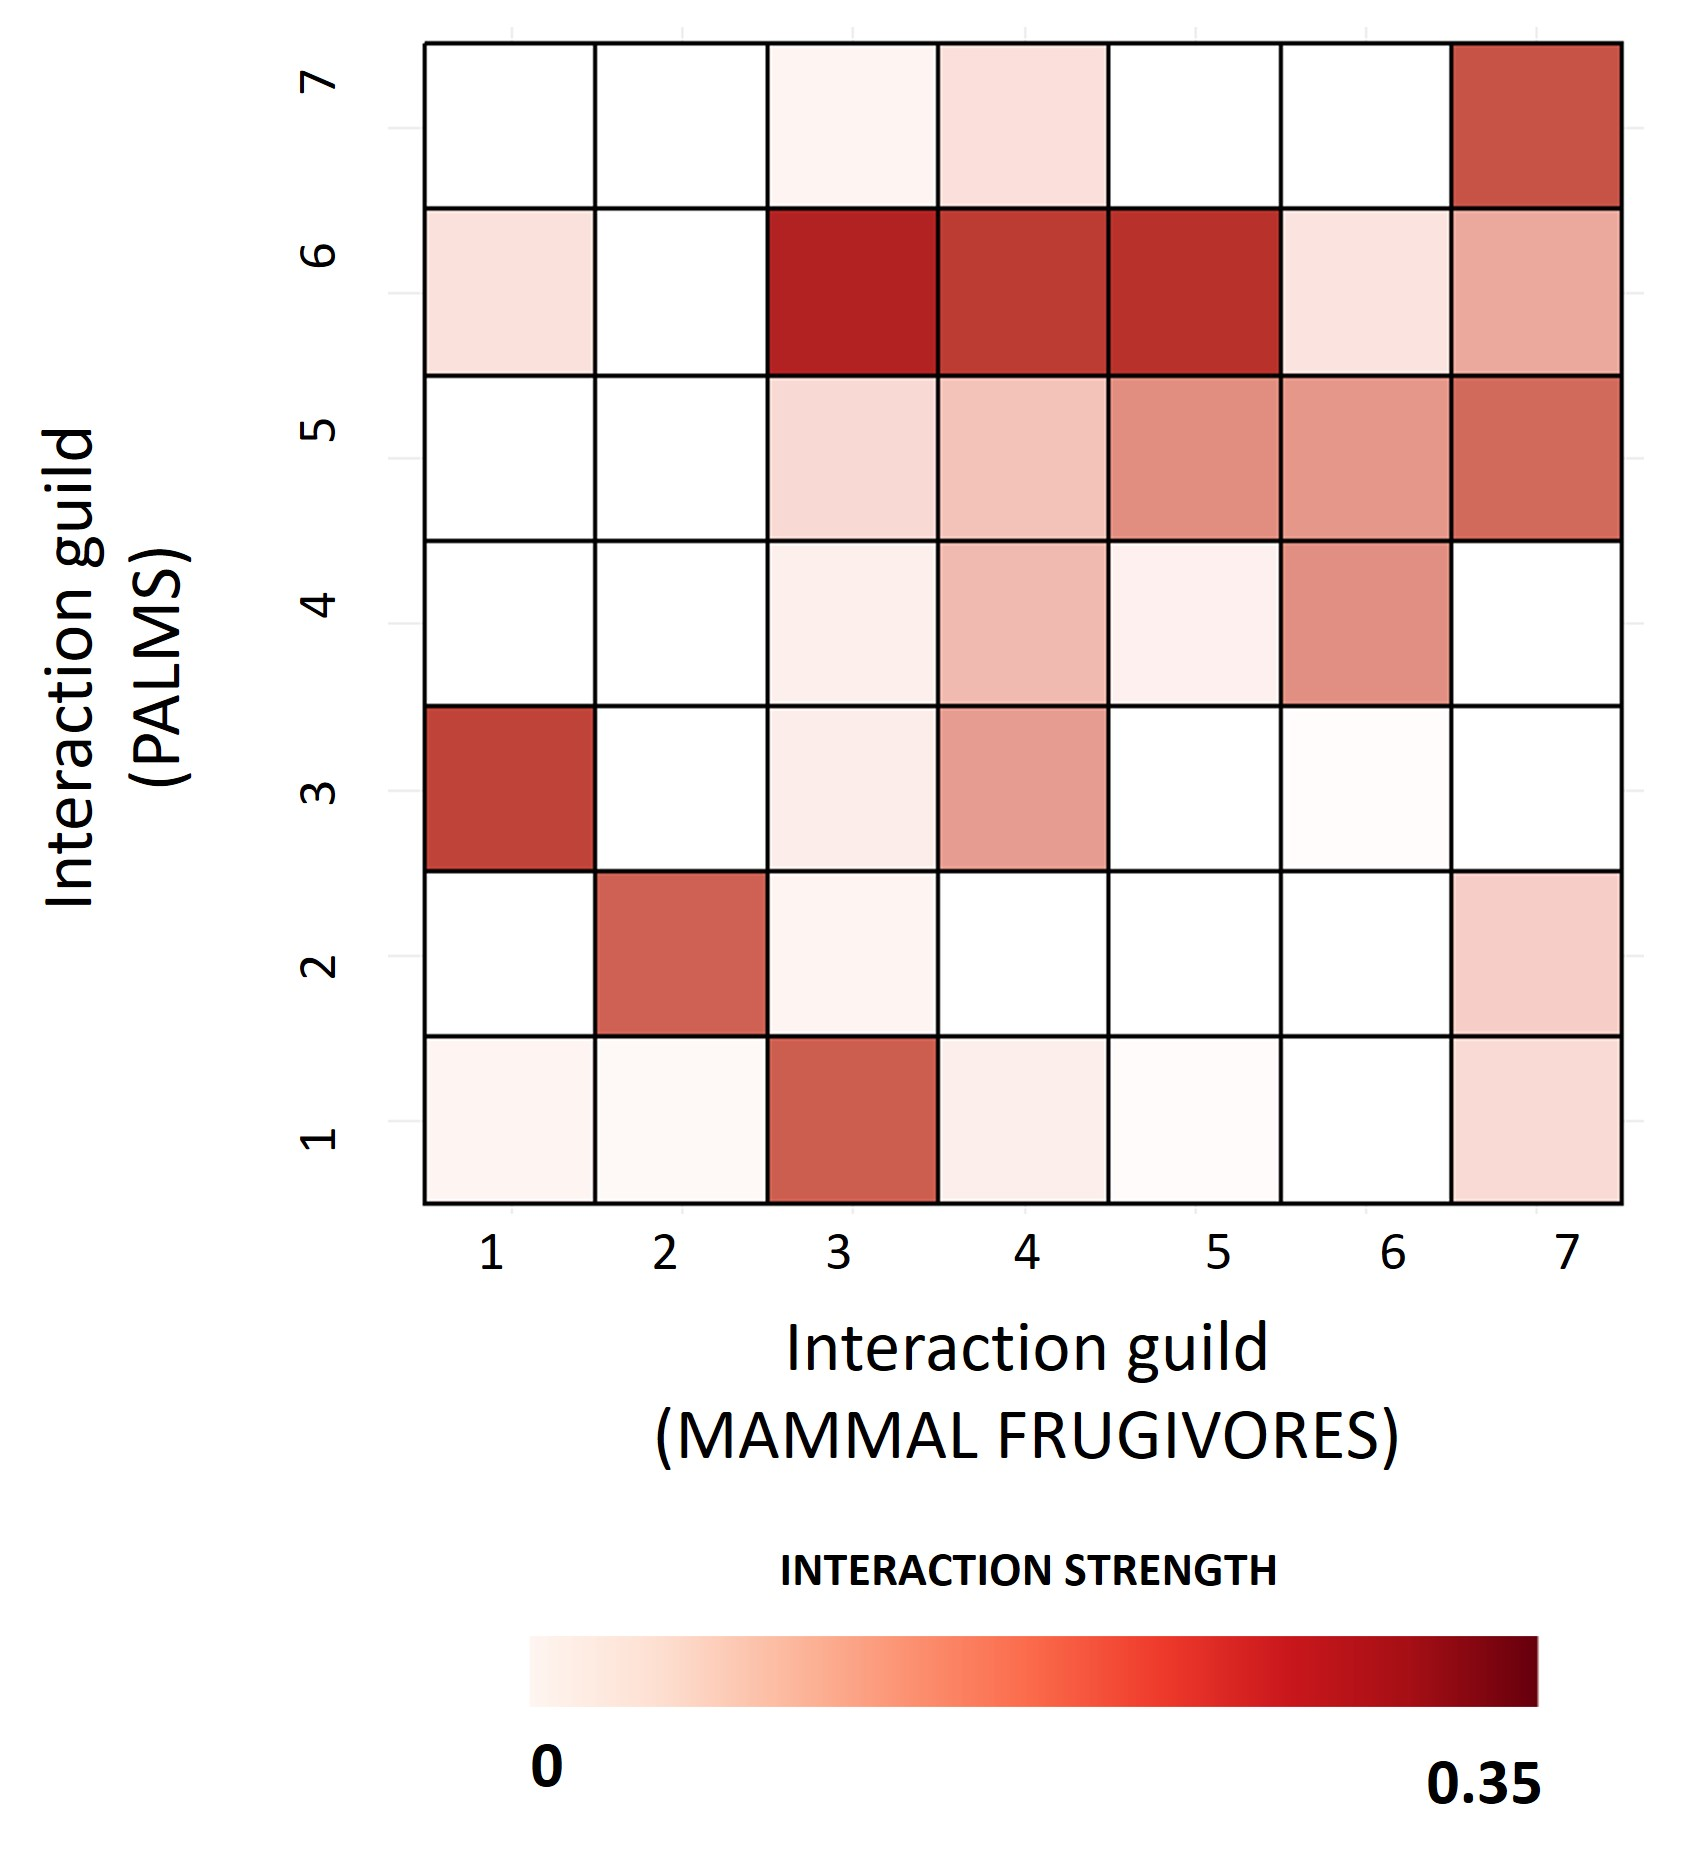
\includegraphics[keepaspectratio]{Main_figures/Picture4.jpg}}

}

\caption{\textbf{Figure 2:} Heatmap depicting the probability of
interaction between palm and mammal interaction guilds defined as blocks
by the Stochastic Block Model (SBM). The intensity of red shading
correlates with the strength of these interactions, where darker shades
signify higher probabilities of interaction between species within or
between interaction guilds (SBM blocks), where the probability was
inferred using the Stochastic Block Model's estimated interaction
parameters (theta Matrix) derived from fitting the model to observed
binary (presence = 1, absence = 0) interaction data compiled from
scientific literature.}

\end{figure}%

\end{footnotesize}}

\subsection{Assessing the influence of climate on functional
richness}\label{assessing-the-influence-of-climate-on-functional-richness}

The GAM results at the assemblage-wide scale show minimal responses in
the functional richness of both palms and mammals to climatic variation
when considered independently of their guild associations (Table S1a,b).
For palms, there is no substantial response to temperature (\emph{F} =
3.00, \emph{P} = 0.00) or precipitation (\emph{F} = 1.19, \emph{P} =
0.23), nor to temperature seasonality (\emph{F} = -0.27, \emph{P} =
0.79) and precipitation seasonality (\emph{F} = 0.68, \emph{P} = 0.50).
Similarly, mammals display mixed responses to environmental factors,
with mean annual temperature showing a strong effect (\emph{F} = 10.60,
\emph{P} = 0.00), while precipitation (F = 0.00, P = 1.00), temperature
seasonality (\emph{F} = 0.52, \emph{P} = 0.60), and precipitation
seasonality (\emph{F} = 1.67, \emph{P} = 0.10) show no significant
effect at the assemblage level.

When incorporating guild into our analyses, generalized additive models
(GAMs) reveal marked differences between trophic levels, particularly in
palms' responses to precipitation seasonality and mammals' responses to
mean annual temperature (Figure S10). For palms, precipitation
seasonality (PS) exhibits significant effects within guilds 5 and 6
(\emph{F} = 5.62, \emph{P} = 0.00 and \emph{F} = 8.37, \emph{P} = 0.01,
respectively), suggesting that these guilds are especially sensitive to
seasonal precipitation variations (Figure S8). In contrast, mammals show
no significant guild-specific response to precipitation seasonality;
instead, their most pronounced response is to temperature, specifically
among species within guild 4 (F = 11.21, \emph{P} = 0.00) (Figure S9).
Notably, guild 3 for mammals and guilds 5 and 6 for palms represent the
dominant guilds across the climatic gradient.

\marginnote{\begin{footnotesize}

\begin{figure}[H]

{\centering \pandocbounded{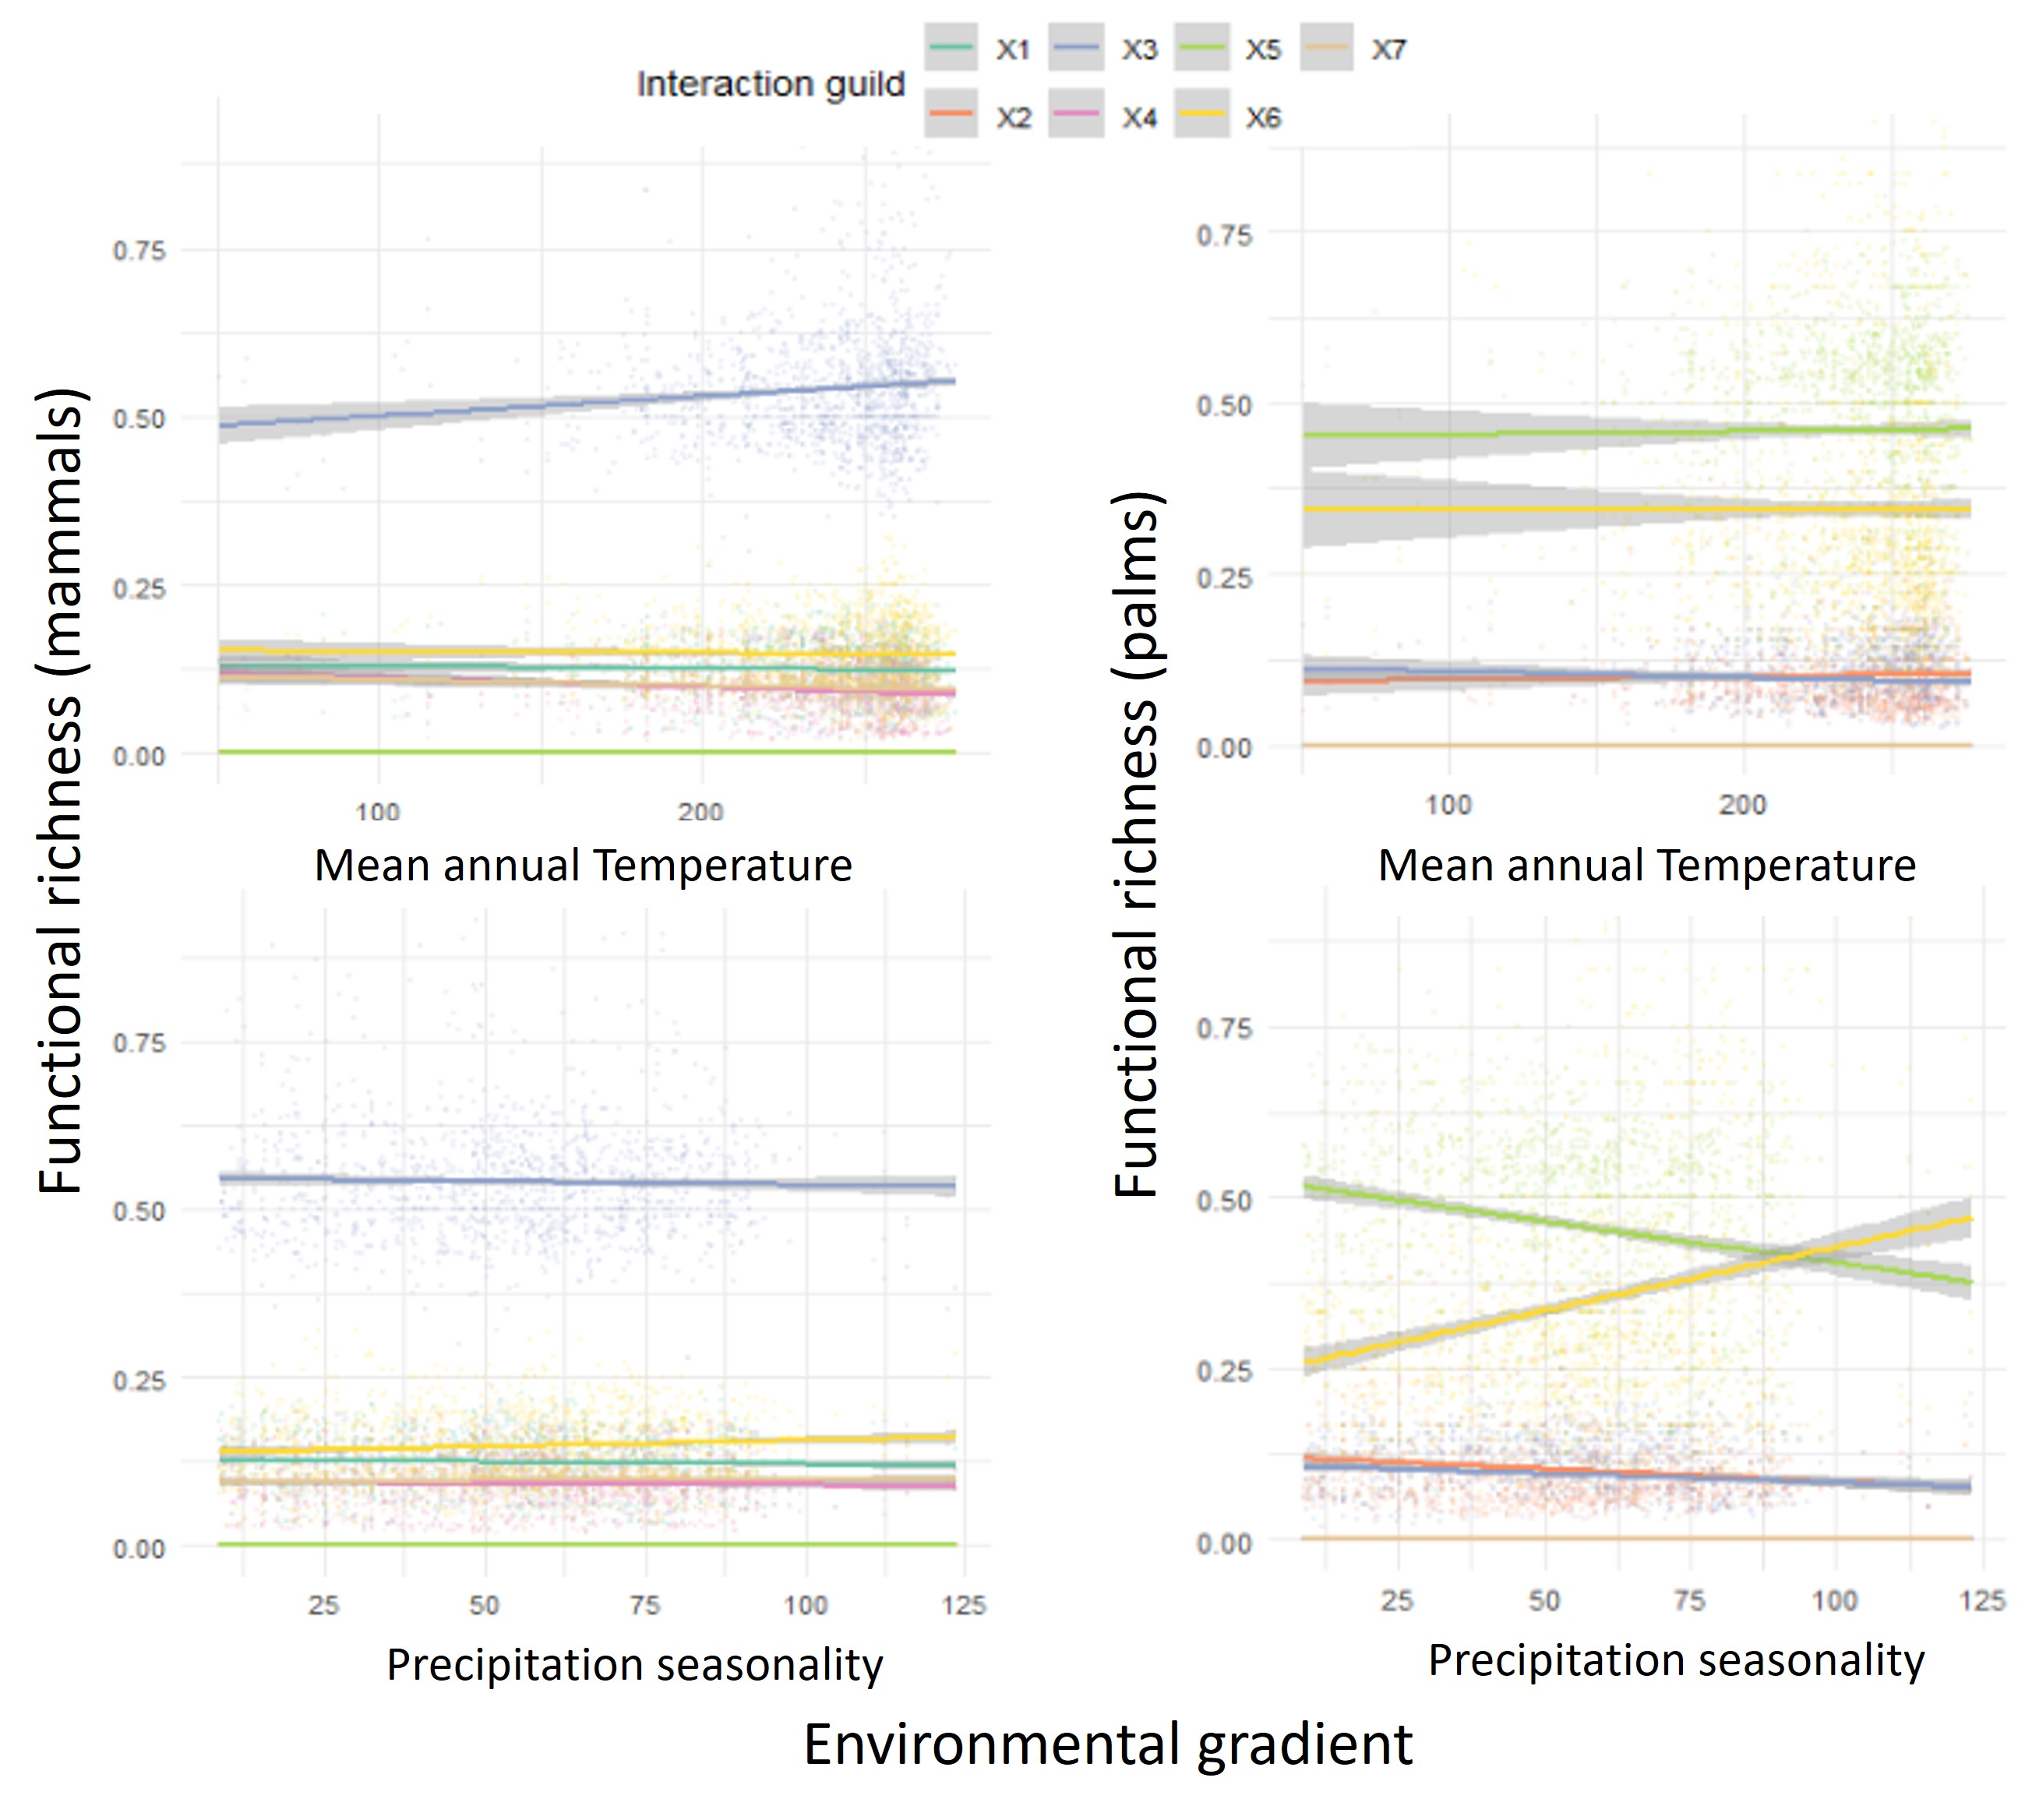
\includegraphics[keepaspectratio]{Main_figures/00_Figure3.png.jpg}}

}

\caption{\textbf{Figure 3:} Functional richness of mammals and palms in
relation to environmental gradients of mean annual temperature and
precipitation seasonality, categorized by interaction guilds (X1 to X7).
Panels on the left illustrate functional richness trends for mammals,
showing varied responses across temperature and precipitation gradients
for each interaction guild. Panels on the right show corresponding
trends for palms. Each line represents a different interaction guild,
with colors indicating distinct guilds as shown in the legend. Points
represent individual observations, while shaded areas around lines
indicate confidence intervals, capturing the variability of functional
richness across environmental conditions.}

\end{figure}%

\end{footnotesize}}

\subsection{Assessing the influence of climate on
FTA}\label{assessing-the-influence-of-climate-on-fta-1}

Interaction strength was identified as the principal non-linear driver
of FTA variation. Our analysis revealed a bi-modal distribution of FTA:
guilds with either high interaction strength (\textgreater{} 0.3) or no
interaction strength ( \textless{} 0.01) exhibited high FTA values,
whereas guilds with moderate interaction strength (0.01 - 0.3) showed
low FTA values.

When incorporating all interaction guilds, the Generalized Additive
Modeling (GAM) analysis reveals a significant effect of mean annual
temperature on functional trophic asymmetry (FTA), with warmer regions
showing elevated FTA values (\emph{F} = 5.97, \emph{P} = 0.01). In this
model, other climate variables, total precipitation, precipitation
seasonality, and temperature seasonality---do not significantly
influence FTA. However, when examining the same GAM model, but excluding
forbidden interactions (i.e.~interaction strength \textless{} 0.01),
both mean annual temperature (\emph{F} = 4.72, \emph{P} = 0.03) and
precipitation seasonality (\emph{F} = 3.95\emph{, P} \textless{} 0.01)
emerge as significant predictors. This refined model suggests that
regions with high mean annual temperatures and high precipitation
seasonality exhibit the highest FTA values. In contrast, regions with
either warm temperatures and low precipitation seasonality or cold
temperatures and high precipitation seasonality are associated with
moderate FTA, while colder regions with low precipitation seasonality
show the lowest FTA values. Notably, temperature seasonality (\emph{F} =
0.01, \emph{P} = 0.91) and total annual precipitation (\emph{F} = 1.68,
\emph{P} = 0.12) remain non-significant in this model.

In analyzing climate effects considering the variation of interaction
strength between consumer and producer guilds, precipitation seasonality
shows a marginally significant effect (\emph{F} = 0.13, \emph{P} =
0.05). After filtering out forbidden interactions, however, the
influence of interaction strength on the effect of precipitation
seasonality becomes non-significant (\emph{F} = 0.00, \emph{P} = 0.09),
while the interaction with total annual precipitation gains statistical
significance (\emph{F} = 0.00, \emph{P} = 0.04), albeit its overall
effect remains low. The model that does not filter by interaction
strength explained a lower proportion of deviance (6.56\%) compared to
model excluding forbidden interactions which accounted for 14.2\% of the
deviance in FTA (Table 1). ~

\marginnote{\begin{footnotesize}

\begin{figure}[H]

{\centering \pandocbounded{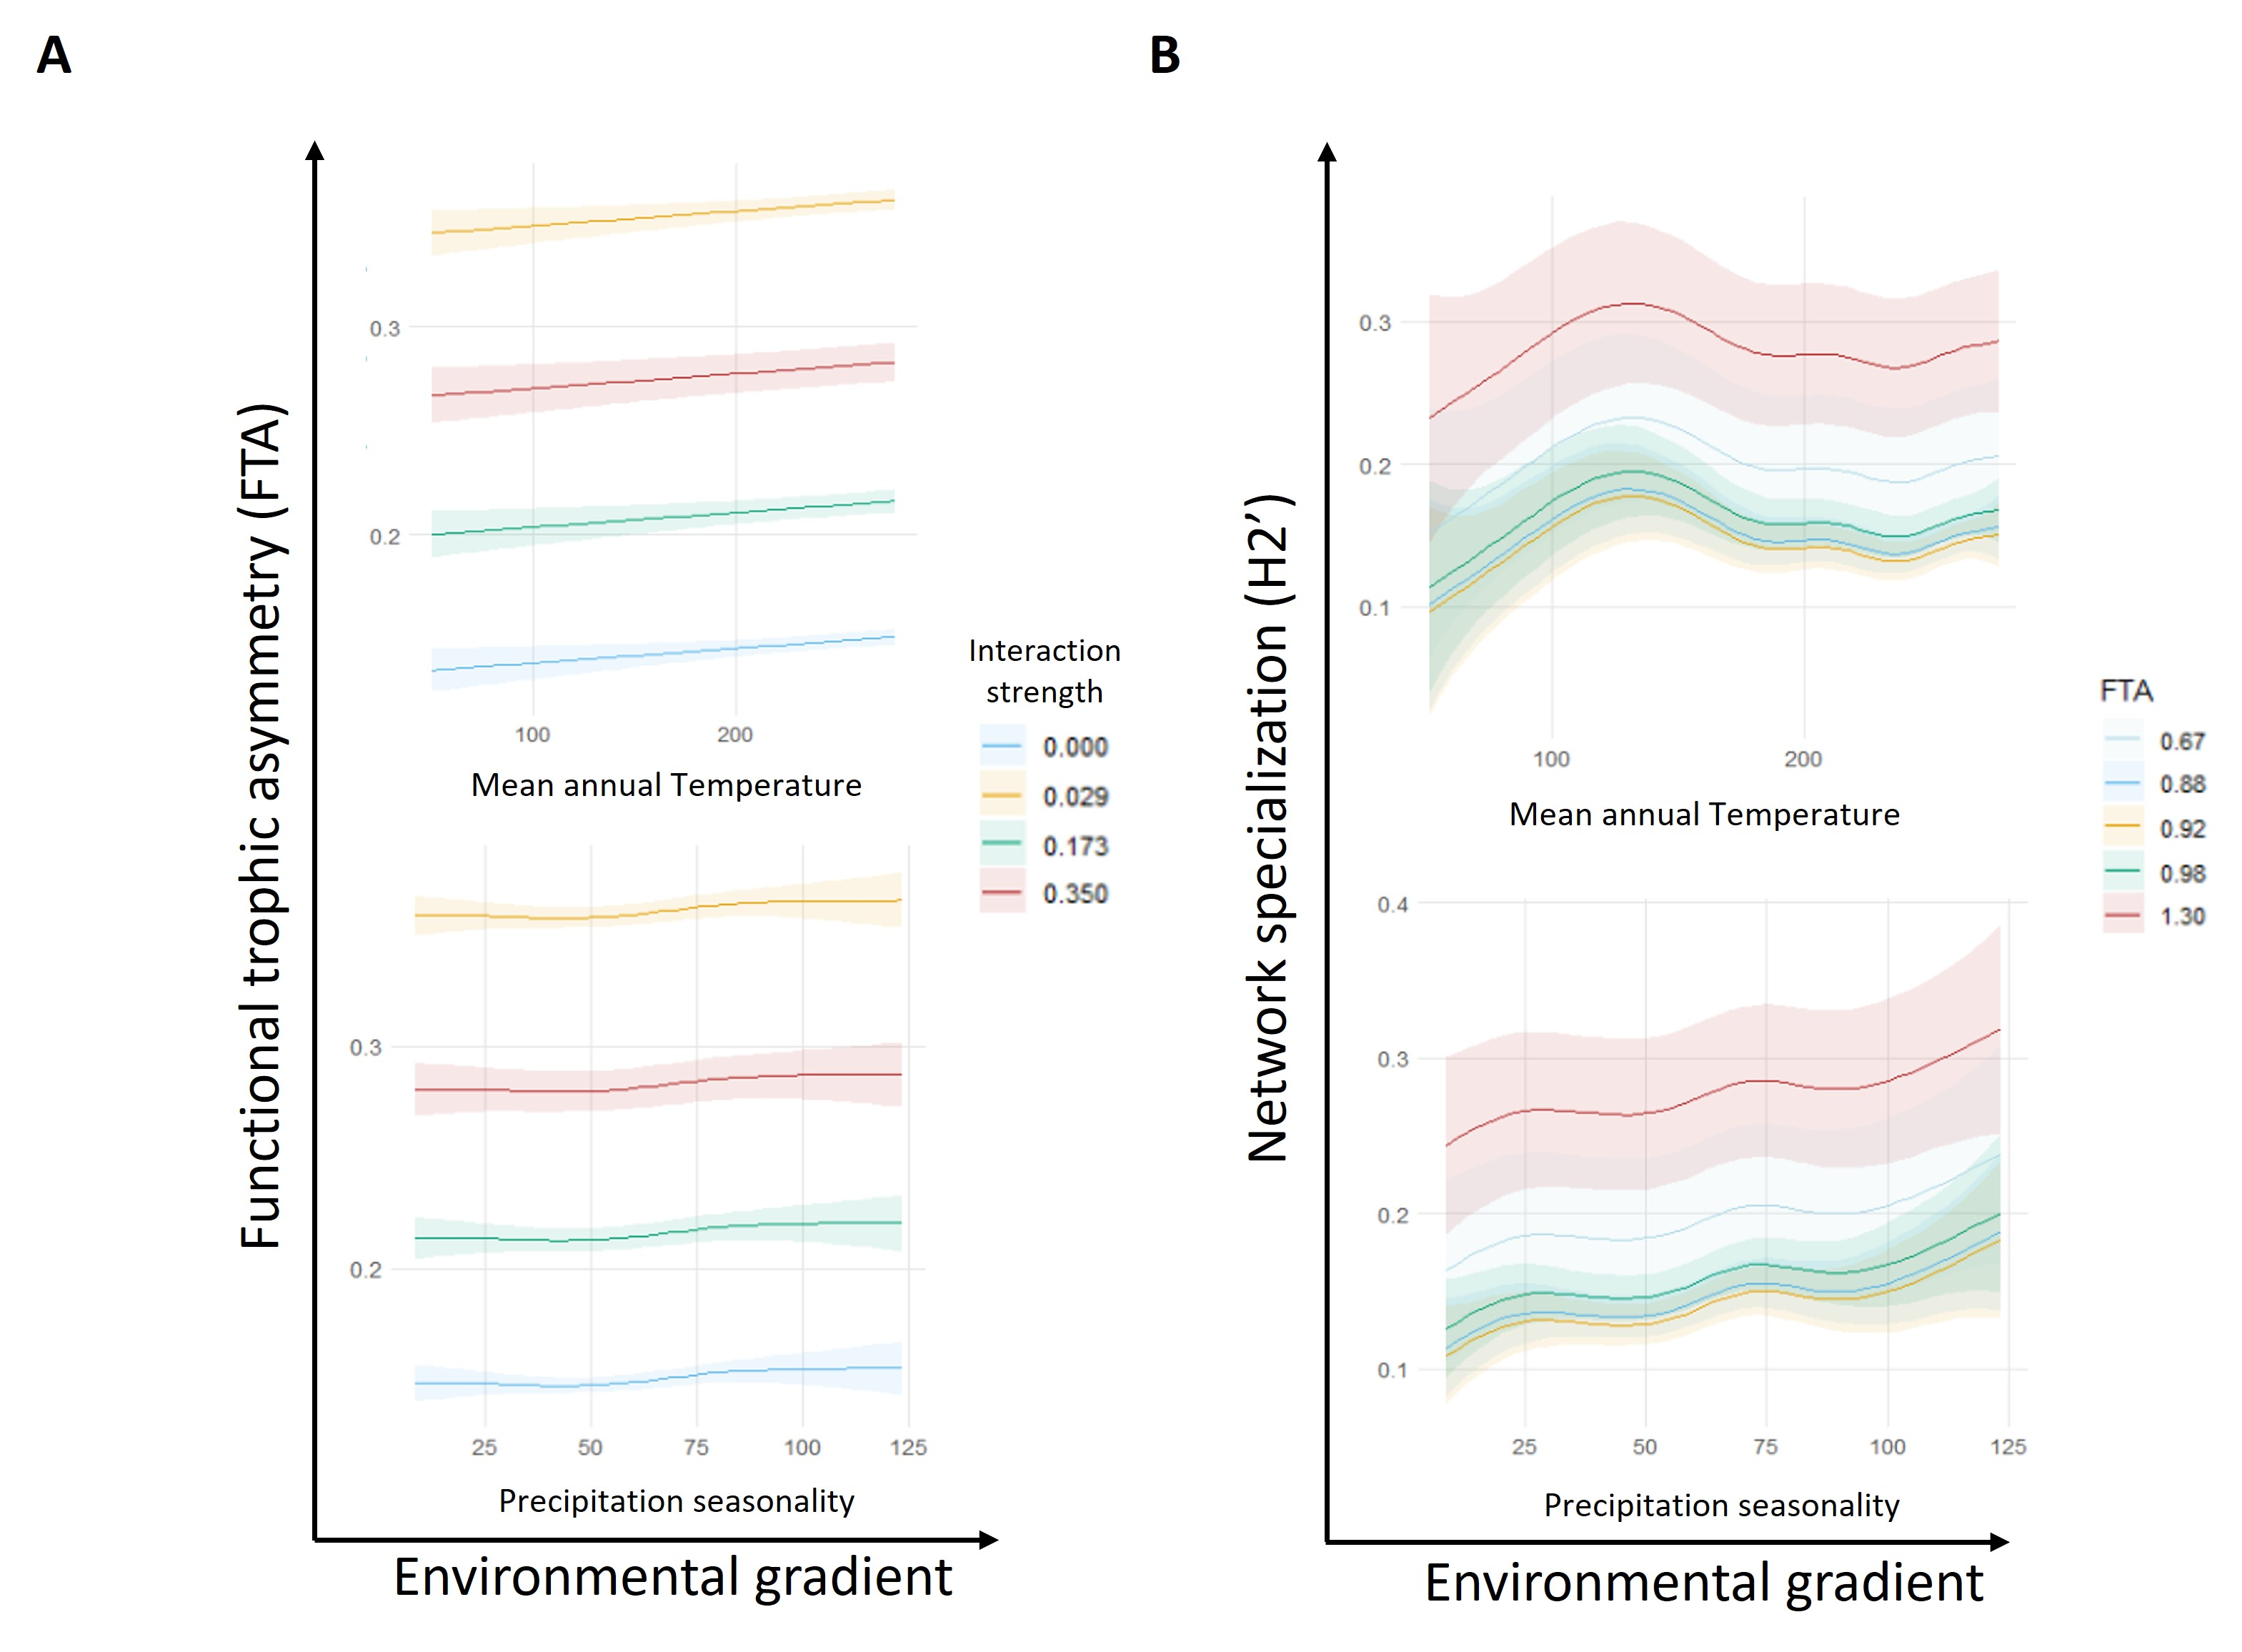
\includegraphics[keepaspectratio]{Main_figures/00_Figure4.png.jpg}}

}

\caption{\textbf{Figure 4:} Functional trophic asymmetry (FTA) and
network specialization (H2') in relation to environmental gradients of
mean annual temperature and precipitation seasonality. Panels on the
left depict the relationship between FTA and environmental gradients,
where lines indicate different levels of interaction strength. Higher
interaction strength (red line) corresponds with increased FTA values.
Panels on the right display network specialization (H2') across the same
environmental gradients, with different levels of FTA represented by
color. Shaded regions indicate confidence intervals, illustrating the
variability across environmental conditions. Arrows at the bottom of
each set of panels represent the direction of the environmental gradient
from low to high values.}

\end{figure}%

\end{footnotesize}}

\subsection{Assessing the relationship between FTA' and
H2'}\label{assessing-the-relationship-between-fta-and-h2-1}

We found that palm-mammalian frugivore networks have levels of trophic
specialization (H2') ranging from 0.12 to 0.25, where 0 means species
have no preference or specialization in their interaction partners and 1
represents networks where each species interacts only with a specific
subset of interaction partners. ~The Generalized Additive Model (GAM)
results indicate that variation in H2' relates most strongly to
variation in FTA' (\emph{F} = 24.36; \emph{P} \textless{} 0.001). Mean
annual temperature also exerts a significant effect (\emph{F} = 2.12,
\emph{P} = 0.03), as does precipitation seasonality PS (\emph{F} = 2.29,
\emph{P} = 0.02) Thus, the model suggests higher specialization in warm
and hot regions with high precipitation seasonality and even higher in
grid cells where multitrophic communities exhibit high functional
trophic asymmetry across all interaction guilds (Figure 4). In contrast,
H2' drops sharply for cold and dry regions, and variation in H2' does
not relate to variation in temperature seasonality or total annual
precipitation ( both \emph{P} \textgreater{} 0.05). The deviance
explained by this model was 17.6\%. ~(Table 2)

\marginnote{\begin{footnotesize}

\begin{figure}[H]

{\centering \pandocbounded{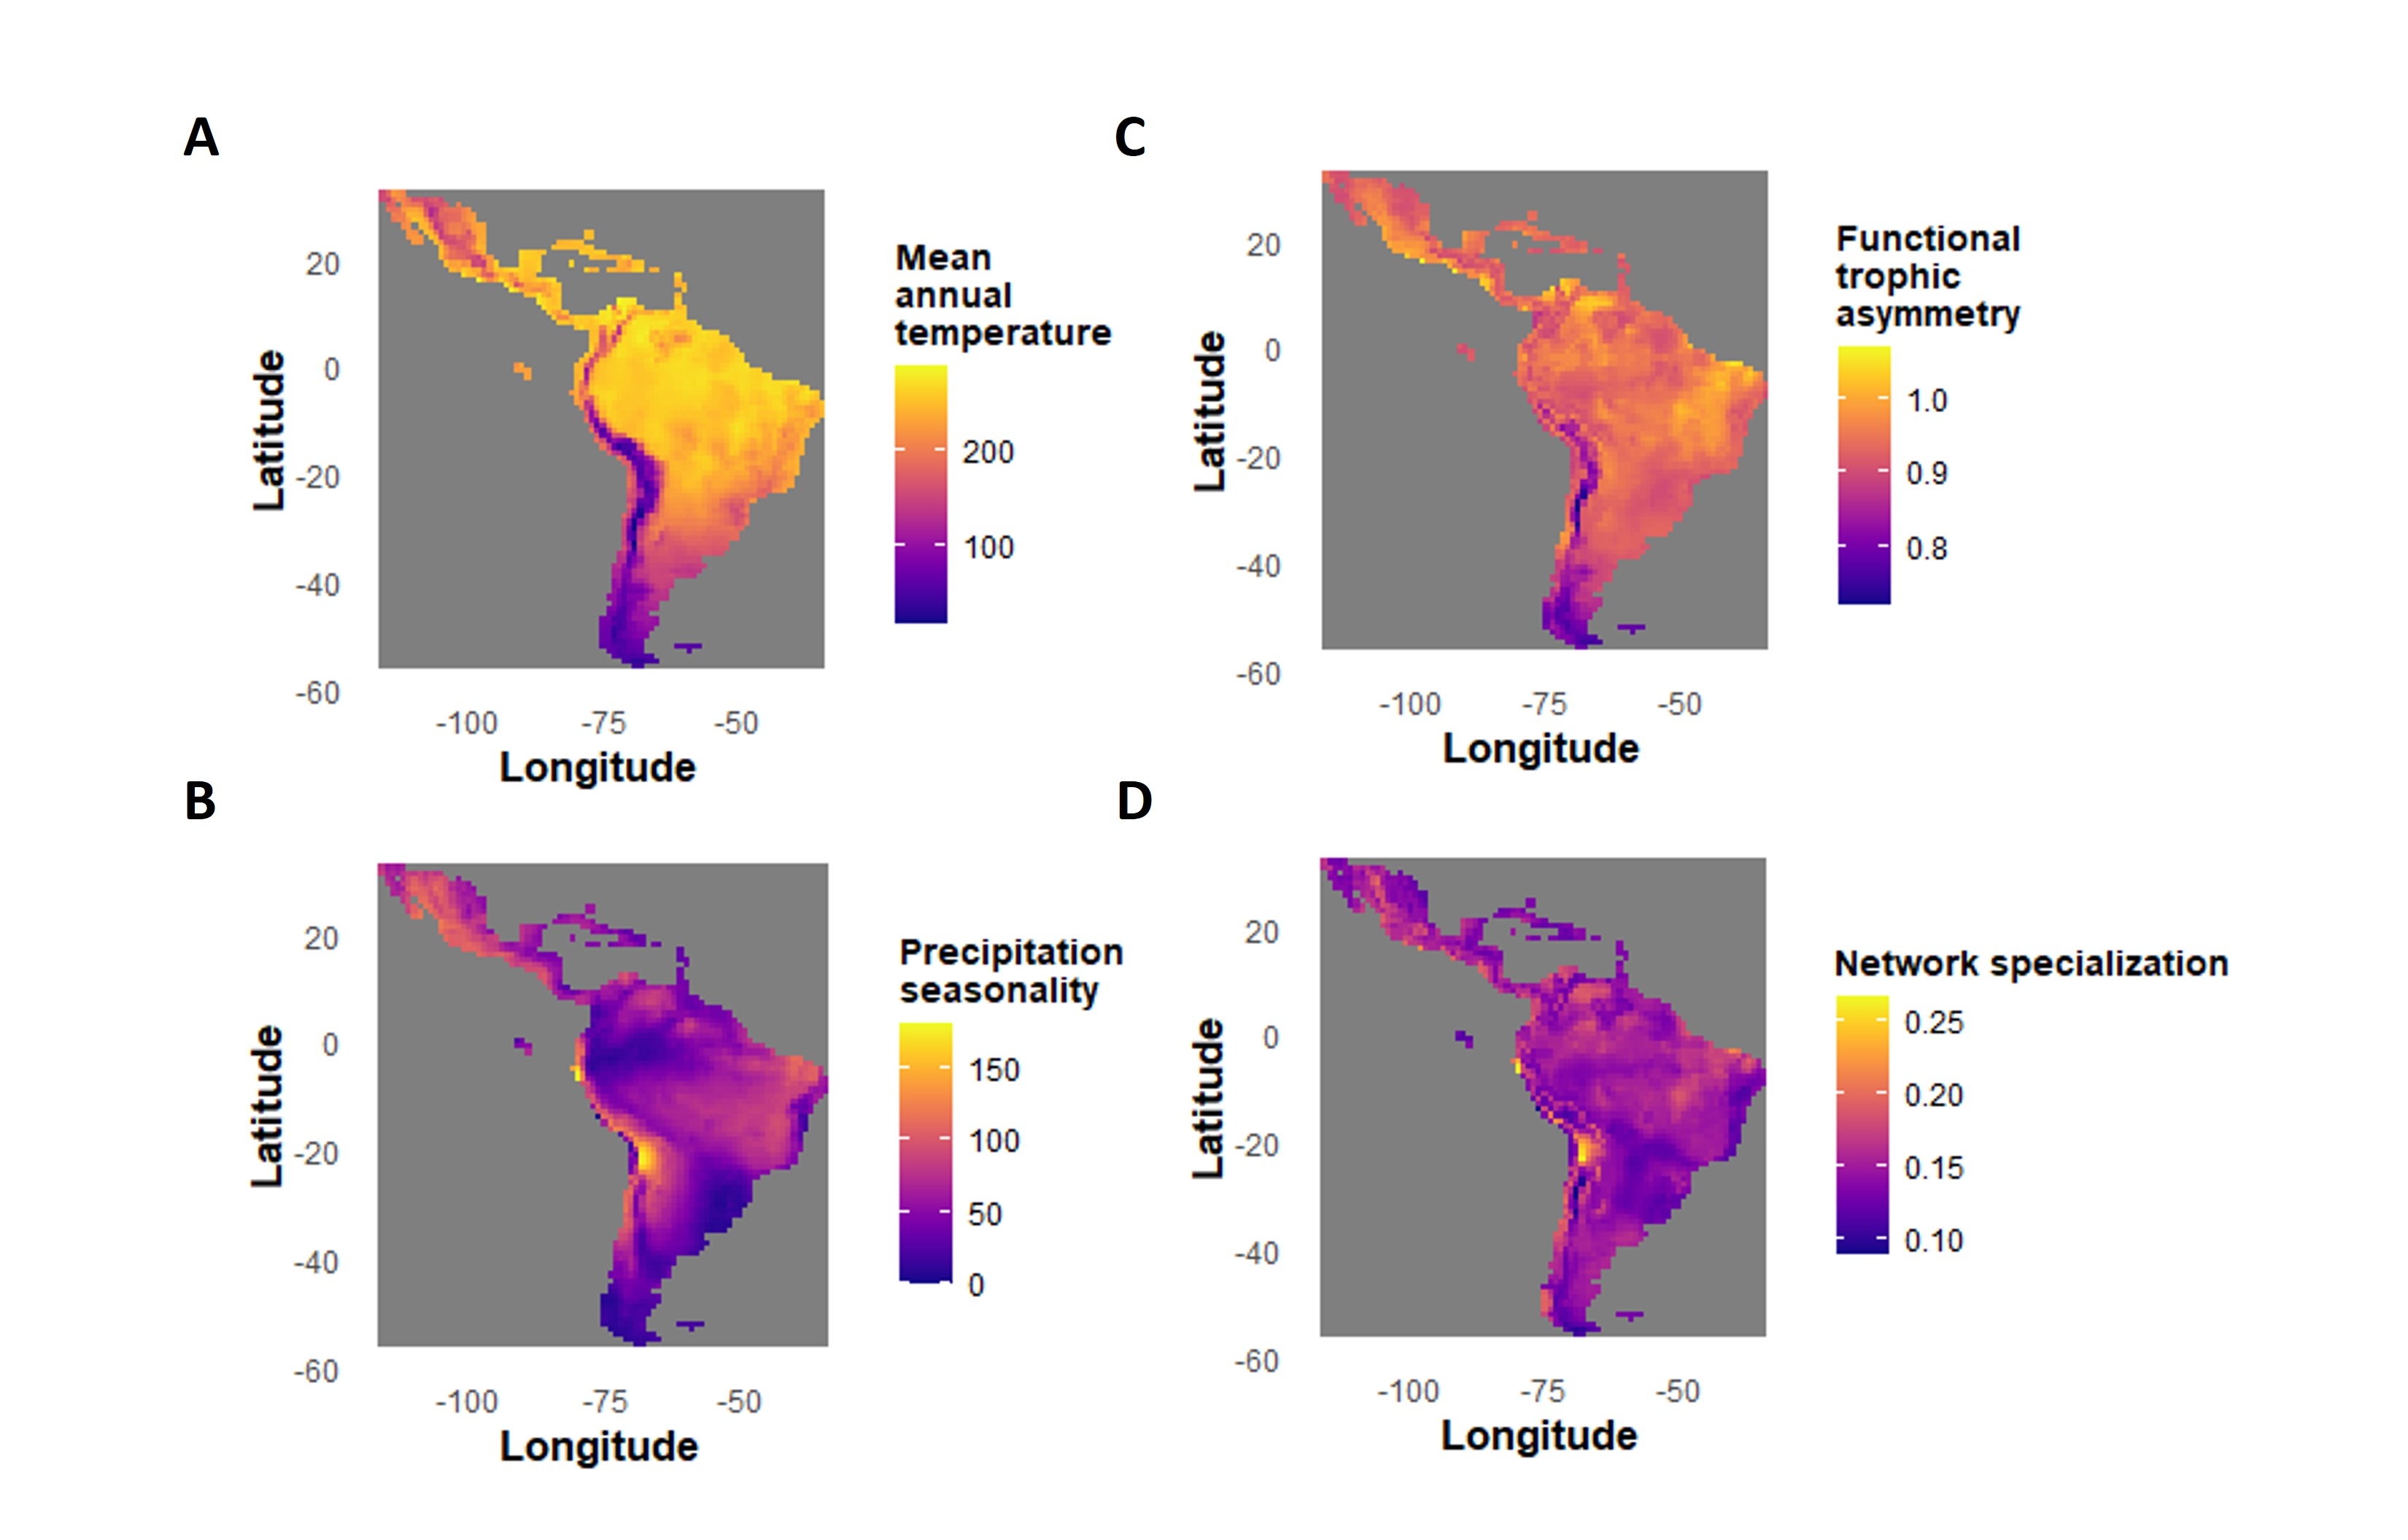
\includegraphics[keepaspectratio]{Main_figures/00_Figure5.png.jpg}}

}

\caption{\textbf{Figure 5:} Spatial distribution of environmental and
ecological variables across the Neotropics. Panels (A) and (B) show the
geographical variation in mean annual temperature and precipitation
seasonality, respectively, with warmer colors indicating higher values.
Panels (C) and (D) depict the spatial patterns of functional trophic
asymmetry (FTA) and network specialization (H2'), where higher values
are also represented by warmer colors. FTA (Panel C) reflects variation
in functional trophic asymmetry across regions, with higher values
concentrated in areas of higher temperature and seasonality. Network
specialization (Panel D) indicates the degree of exclusive interactions
within ecological networks. Color scales for each map are shown in
adjacent legends.}

\end{figure}%

\end{footnotesize}}

\section{References}\label{references}

\section{Tables}\label{tables}

Table 1a: Summary of parametric and smooth term coefficients for models
predicting FTA responses to climate for all guilds. The parametric
coefficients include estimates, standard errors, t-values, and p-values
for the intercept. Smooth terms are presented for each predictor and its
interactions, showing effective degrees of freedom (edf), reference
degrees of freedom (Ref.df), F-statistics, and p-values under both
conditions. Significant p-values highlight predictors or interactions
with a statistically significant effect.

\begin{longtable}[]{@{}
  >{\centering\arraybackslash}p{(\linewidth - 8\tabcolsep) * \real{0.2000}}
  >{\centering\arraybackslash}p{(\linewidth - 8\tabcolsep) * \real{0.2000}}
  >{\centering\arraybackslash}p{(\linewidth - 8\tabcolsep) * \real{0.2000}}
  >{\centering\arraybackslash}p{(\linewidth - 8\tabcolsep) * \real{0.2000}}
  >{\centering\arraybackslash}p{(\linewidth - 8\tabcolsep) * \real{0.2000}}@{}}
\toprule\noalign{}
\endhead
\bottomrule\noalign{}
\endlastfoot
~ &
\multicolumn{4}{>{\centering\arraybackslash}p{(\linewidth - 8\tabcolsep) * \real{0.8000} + 6\tabcolsep}@{}}{%
Dependent variable} \\
Predictors & Estimates & std. Error & CI & p \\
(Intercept) & 0.21 & 0.00 & 0.21~--~0.21 & \textbf{\textless0.001} \\
Smooth term (Temp) & & & & \textbf{0.007} \\
\begin{minipage}[t]{\linewidth}\raggedright
Smooth term (Temp,int\\
str)\strut
\end{minipage} & & & & 0.383 \\
Smooth term (PS) & & & & 0.636 \\
Smooth term (PS,int str) & & & & \textbf{0.030} \\
Smooth term (TS) & & & & 0.763 \\
Smooth term (TS,int str) & & & & 0.421 \\
Smooth term (Prec) & & & & 0.776 \\
\begin{minipage}[t]{\linewidth}\raggedright
Smooth term (Prec,int\\
str)\strut
\end{minipage} & & & & 0.289 \\
Smooth term (int str) & & & & \textbf{\textless0.001} \\
Observations &
\multicolumn{4}{>{\raggedright\arraybackslash}p{(\linewidth - 8\tabcolsep) * \real{0.8000} + 6\tabcolsep}@{}}{%
53406} \\
R\textsuperscript{2} &
\multicolumn{4}{>{\raggedright\arraybackslash}p{(\linewidth - 8\tabcolsep) * \real{0.8000} + 6\tabcolsep}@{}}{%
0.200} \\
\end{longtable}

\textsubscript{Source:
\href{https://lessardlab.github.io/FTA-Neotropics/index.qmd.html}{Article
Notebook}}

Table 1b: Summary of parametric and smooth term coefficients for models
predicting FTA responses to climate for guilds with interaction
probabilities \textgreater{} 0.01. The parametric coefficients include
estimates, standard errors, t-values, and p-values for the intercept.
Smooth terms are presented for each predictor and its interactions,
showing effective degrees of freedom (edf), reference degrees of freedom
(Ref.df), F-statistics, and p-values under both conditions. Significant
p-values highlight predictors or interactions with a statistically
significant effect.

\begin{longtable}[]{@{}
  >{\centering\arraybackslash}p{(\linewidth - 8\tabcolsep) * \real{0.2000}}
  >{\centering\arraybackslash}p{(\linewidth - 8\tabcolsep) * \real{0.2000}}
  >{\centering\arraybackslash}p{(\linewidth - 8\tabcolsep) * \real{0.2000}}
  >{\centering\arraybackslash}p{(\linewidth - 8\tabcolsep) * \real{0.2000}}
  >{\centering\arraybackslash}p{(\linewidth - 8\tabcolsep) * \real{0.2000}}@{}}
\toprule\noalign{}
\endhead
\bottomrule\noalign{}
\endlastfoot
~ &
\multicolumn{4}{>{\centering\arraybackslash}p{(\linewidth - 8\tabcolsep) * \real{0.8000} + 6\tabcolsep}@{}}{%
Dependent variable} \\
Predictors & Estimates & std. Error & CI & p \\
(Intercept) & 0.25 & 0.00 & 0.24~--~0.25 & \textbf{\textless0.001} \\
Smooth term (Temp) & & & & \textbf{0.028} \\
\begin{minipage}[t]{\linewidth}\raggedright
Smooth term (Temp,int\\
str)\strut
\end{minipage} & & & & 0.068 \\
Smooth term (PS) & & & & \textbf{0.004} \\
Smooth term (PS,int str) & & & & 0.063 \\
Smooth term (TS) & & & & 0.876 \\
Smooth term (TS,int str) & & & & 0.506 \\
Smooth term (Prec) & & & & 0.098 \\
\begin{minipage}[t]{\linewidth}\raggedright
Smooth term (Prec,int\\
str)\strut
\end{minipage} & & & & \textbf{0.042} \\
Smooth term (int str) & & & & \textbf{\textless0.001} \\
Observations &
\multicolumn{4}{>{\raggedright\arraybackslash}p{(\linewidth - 8\tabcolsep) * \real{0.8000} + 6\tabcolsep}@{}}{%
33534} \\
R\textsuperscript{2} &
\multicolumn{4}{>{\raggedright\arraybackslash}p{(\linewidth - 8\tabcolsep) * \real{0.8000} + 6\tabcolsep}@{}}{%
0.206} \\
\end{longtable}

\textsubscript{Source:
\href{https://lessardlab.github.io/FTA-Neotropics/index.qmd.html}{Article
Notebook}}

Table 2: Summary of parametric and smooth term coefficients for the
model predicting H2' responses based on environmental and FTA variables.
The parametric coefficients include the estimate, standard error,
t-value, and p-value for the intercept. Smooth terms are shown for each
predictor (sum\_fta, Temp, PS, TS, and Prec), providing the effective
degrees of freedom (edf), reference degrees of freedom (Ref.df),
F-statistics, and p-values, which indicate the statistical significance
of each smooth term. Significant p-values suggest predictors with a
meaningful contribution to the model.

\begin{longtable}[]{@{}ccccc@{}}
\toprule\noalign{}
\endhead
\bottomrule\noalign{}
\endlastfoot
~ & \multicolumn{4}{c@{}}{%
Dependent variable} \\
Predictors & Estimates & std. Error & CI & p \\
(Intercept) & 0.16 & 0.00 & 0.16~--~0.17 & \textbf{\textless0.001} \\
Smooth term (sum fta) & & & & \textbf{\textless0.001} \\
Smooth term (Temp) & & & & \textbf{0.040} \\
Smooth term (PS) & & & & \textbf{0.029} \\
Smooth term (TS) & & & & 0.391 \\
Smooth term (Prec) & & & & 0.482 \\
Observations & \multicolumn{4}{l@{}}{%
1242} \\
R\textsuperscript{2} & \multicolumn{4}{l@{}}{%
0.160} \\
\end{longtable}

\textsubscript{Source:
\href{https://lessardlab.github.io/FTA-Neotropics/index.qmd.html}{Article
Notebook}}

\section{Supplementary Figures}\label{supplementary-figures}

\subsection{Supplementary Figure 1}

\begin{figure}[H]

{\centering 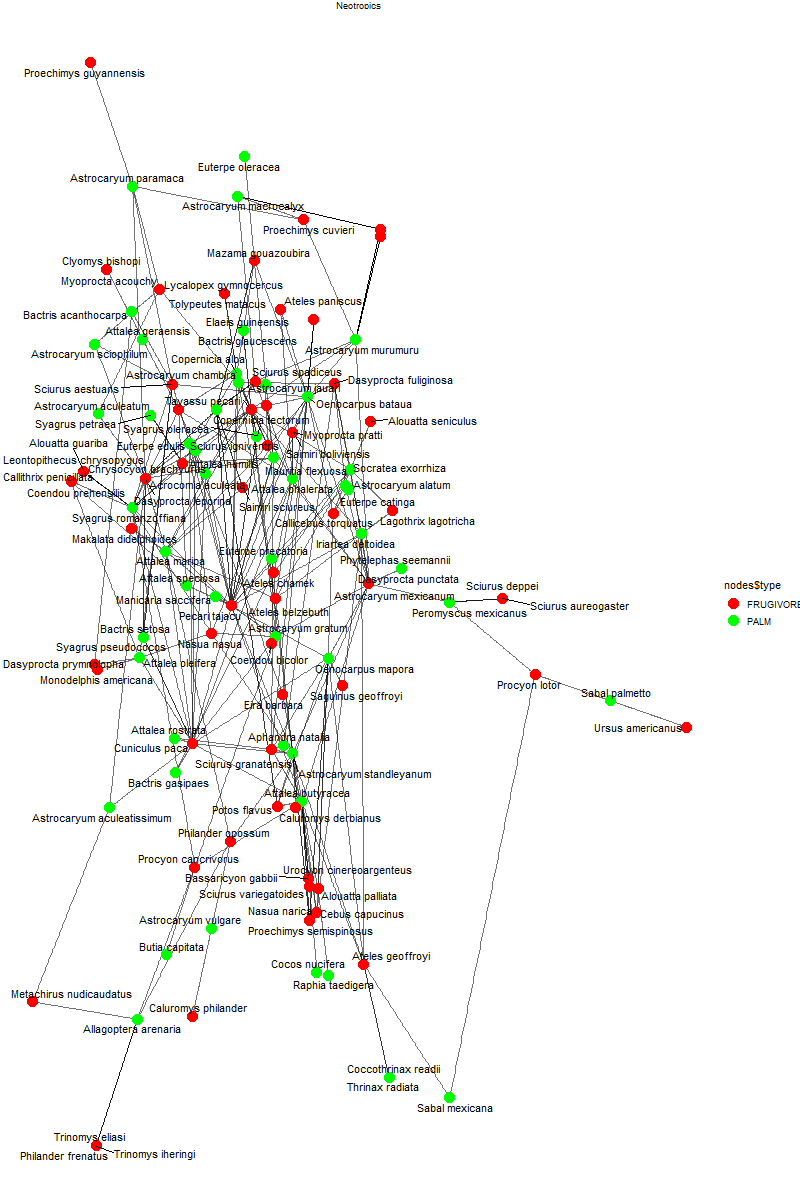
\includegraphics[width=5.64583in,height=\textheight,keepaspectratio]{sup_figures/S1_metaweb.png}

}

\caption{Metaweb of interactions}

\end{figure}%

\subsection{Supplementary Figure 2}

\begin{figure}[H]

{\centering 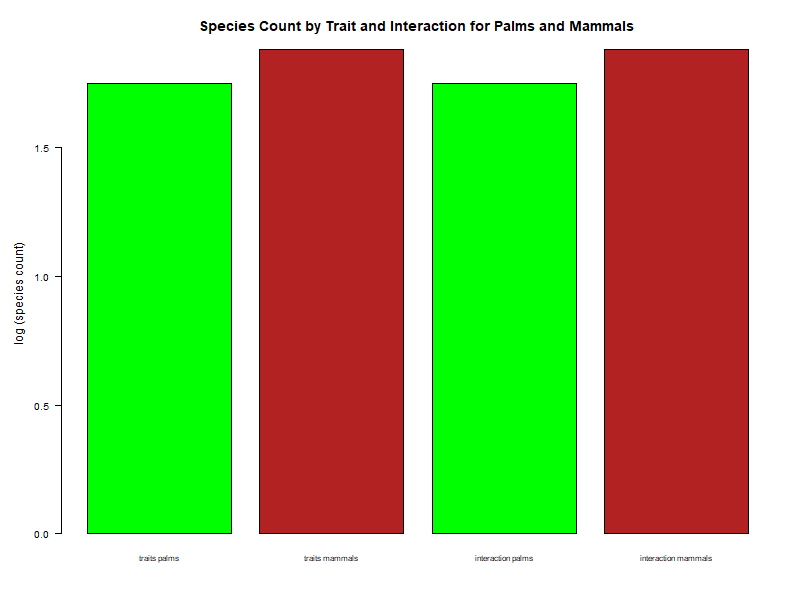
\includegraphics[width=5.67708in,height=\textheight,keepaspectratio]{sup_figures/species_count_plot_AAS_style.png}

}

\caption{Data imbalance}

\end{figure}%

\subsection{Supplementary Figure 3}

\begin{figure}[H]

{\centering 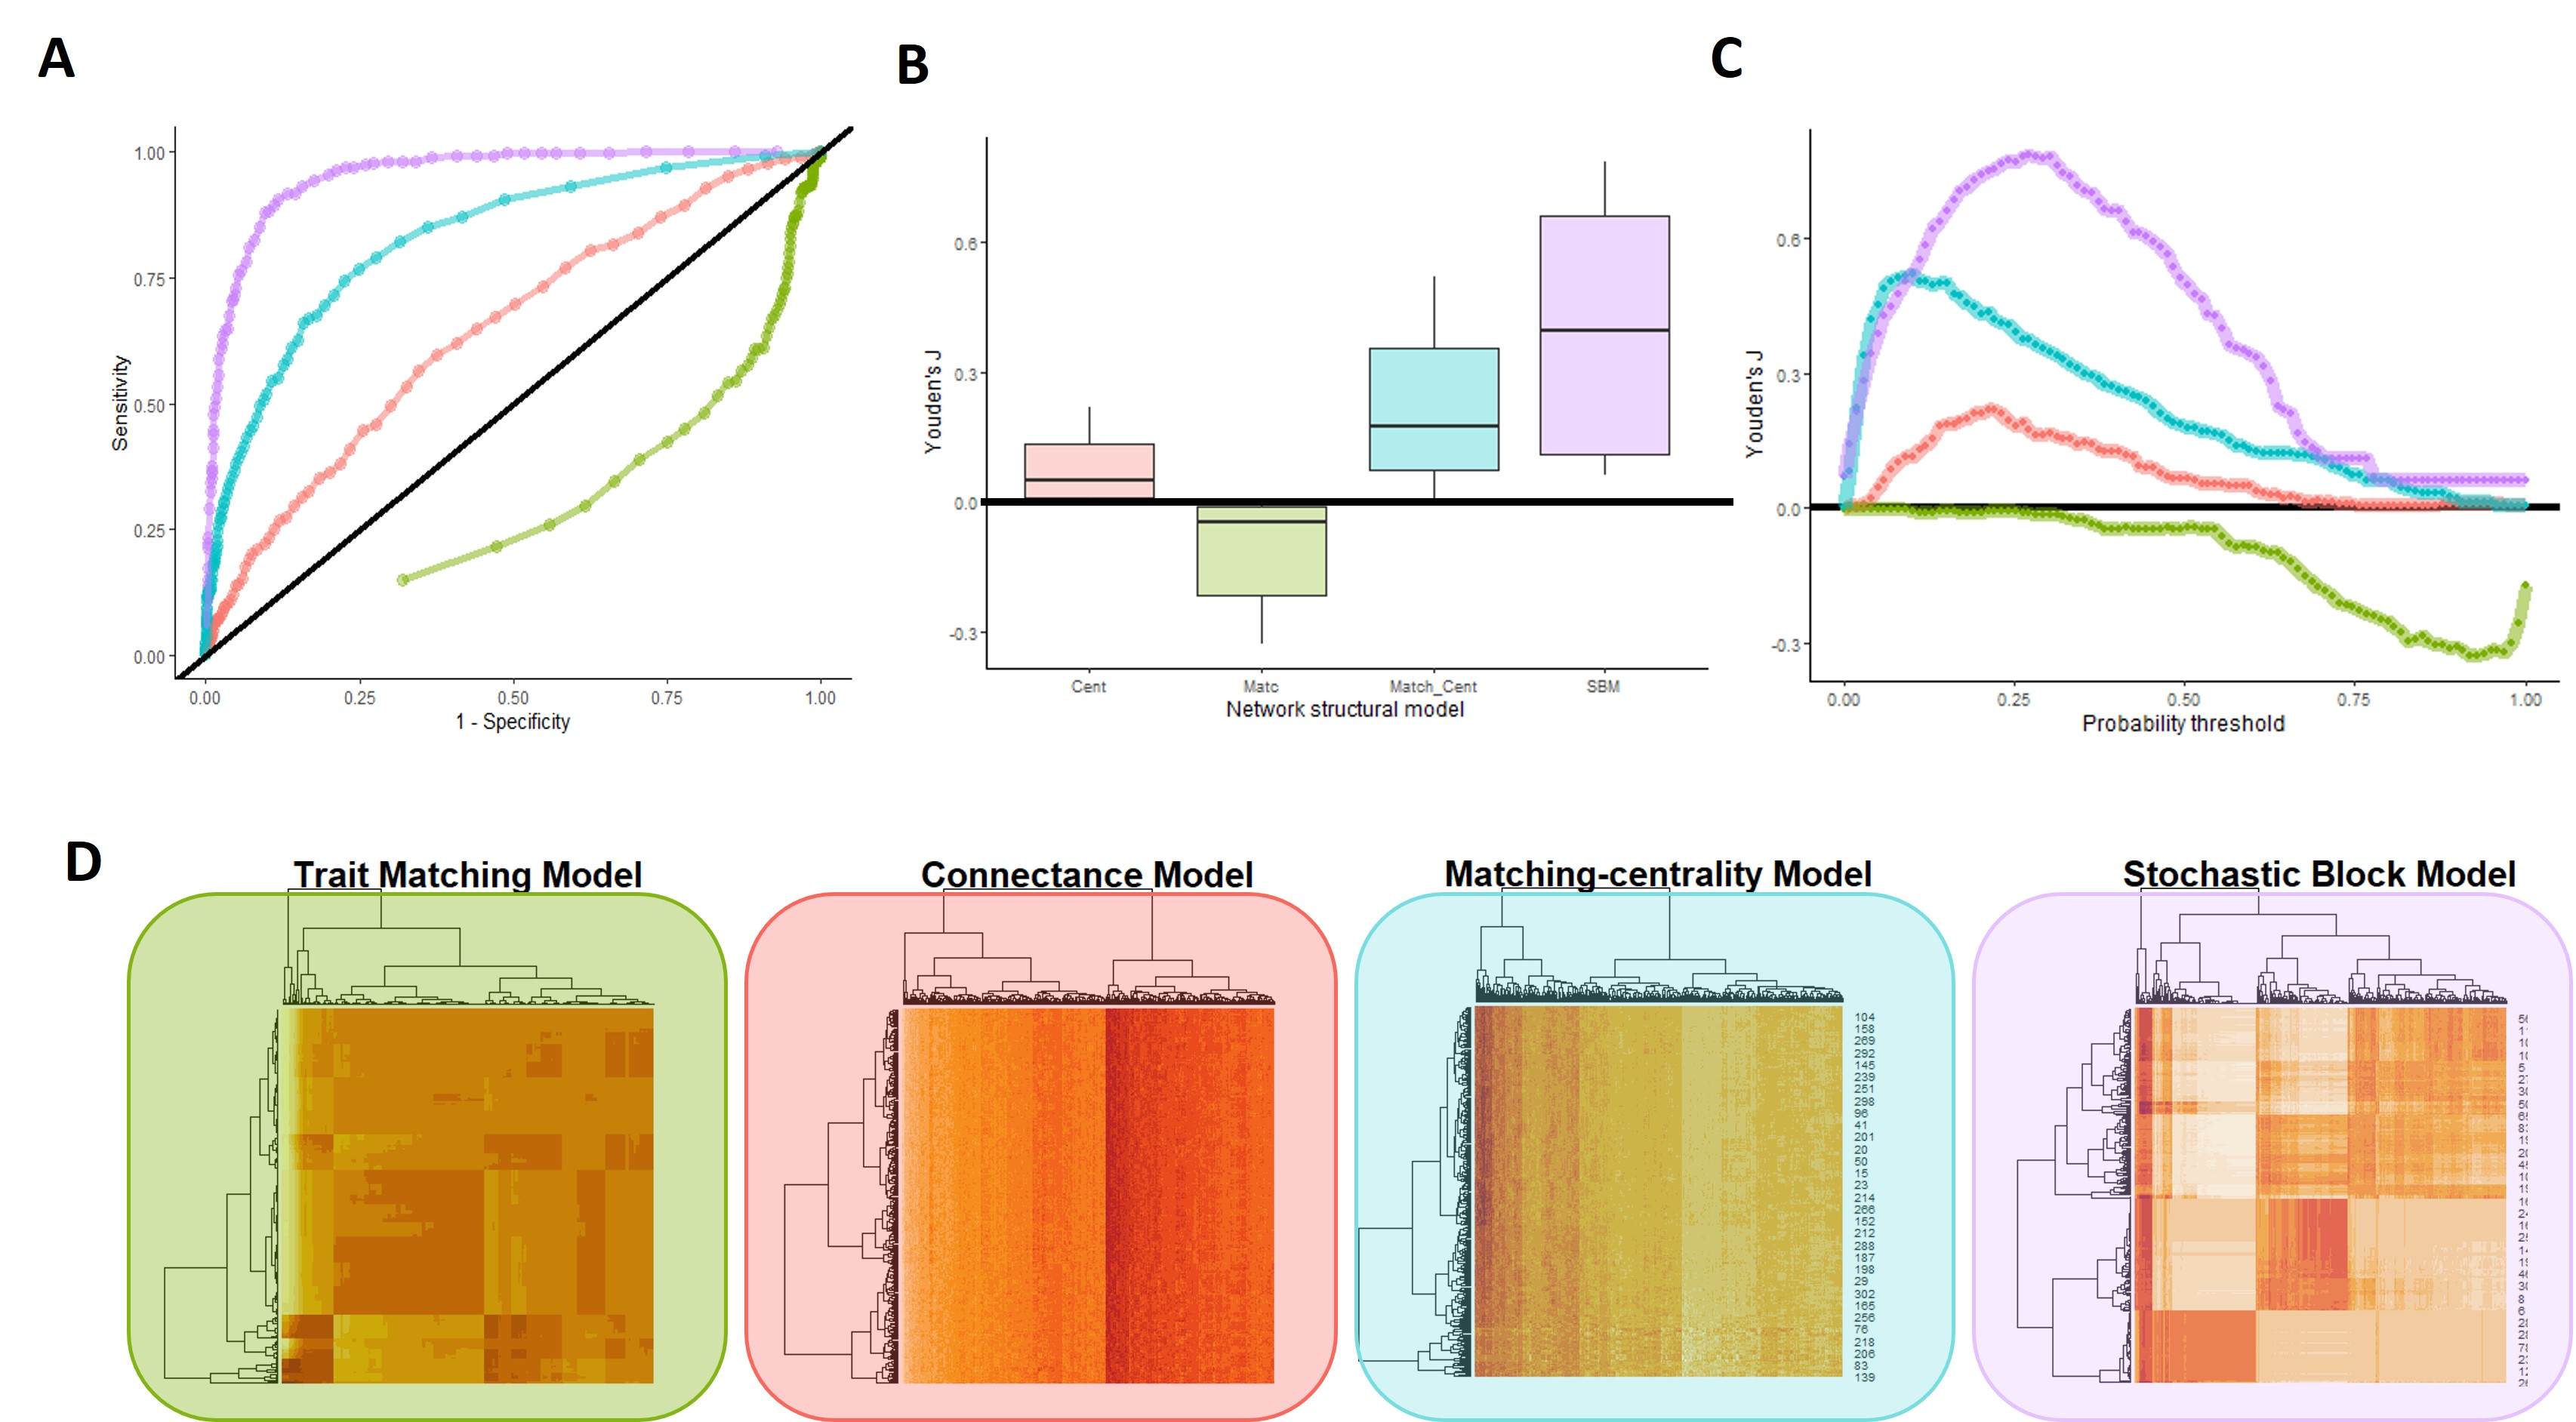
\includegraphics[width=5.67708in,height=\textheight,keepaspectratio]{sup_figures/Sup_modelsfit.jpg}

}

\caption{Latent network model fit}

\end{figure}%

\subsection{Supplementary Figure 4}

\begin{figure}[H]

{\centering 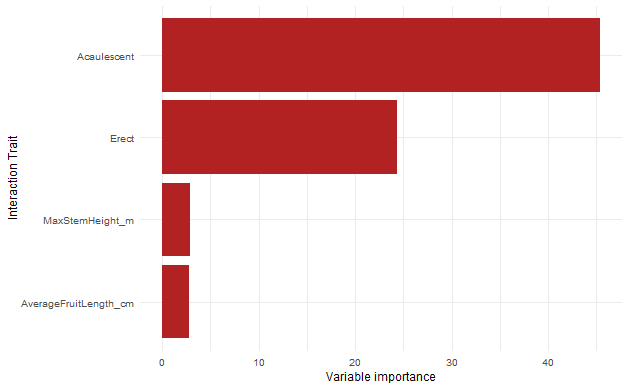
\includegraphics[width=5.67708in,height=\textheight,keepaspectratio]{sup_figures/palm_var_imp.jpg}

}

\caption{Data imbalance}

\end{figure}%

\subsection{Supplementary Figure 5}

\begin{figure}[H]

{\centering 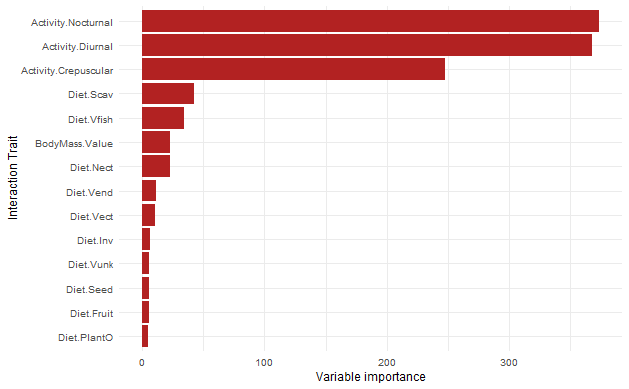
\includegraphics[width=5.67708in,height=\textheight,keepaspectratio]{sup_figures/mammal_var_imp.jpg}

}

\caption{Data imbalance}

\end{figure}%

\subsection{Supplementary Figure 6}

\begin{figure}[H]

{\centering 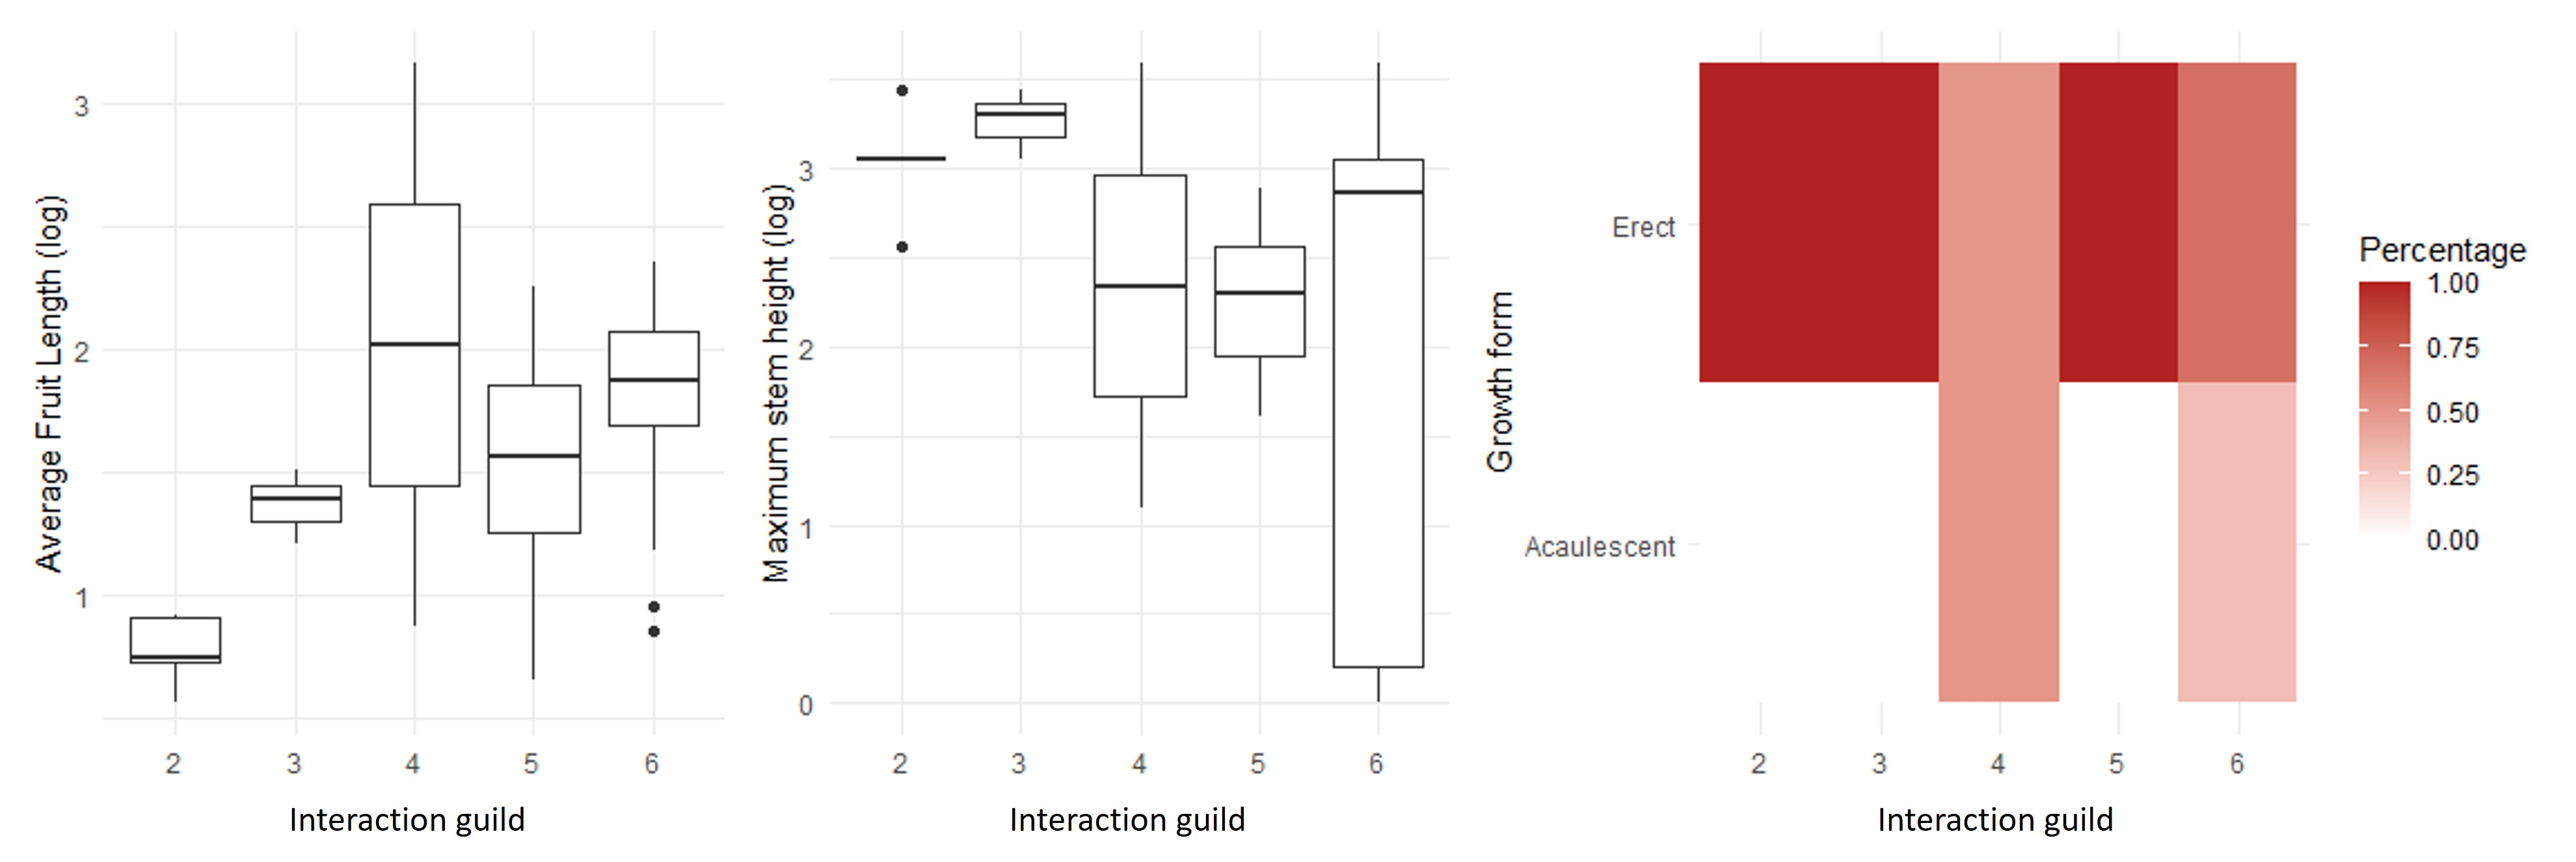
\includegraphics[width=5.67708in,height=\textheight,keepaspectratio]{sup_figures/palm_trait_sbm.jpg}

}

\caption{Data imbalance}

\end{figure}%

\subsection{Supplementary Figure 7}

\begin{figure}[H]

{\centering 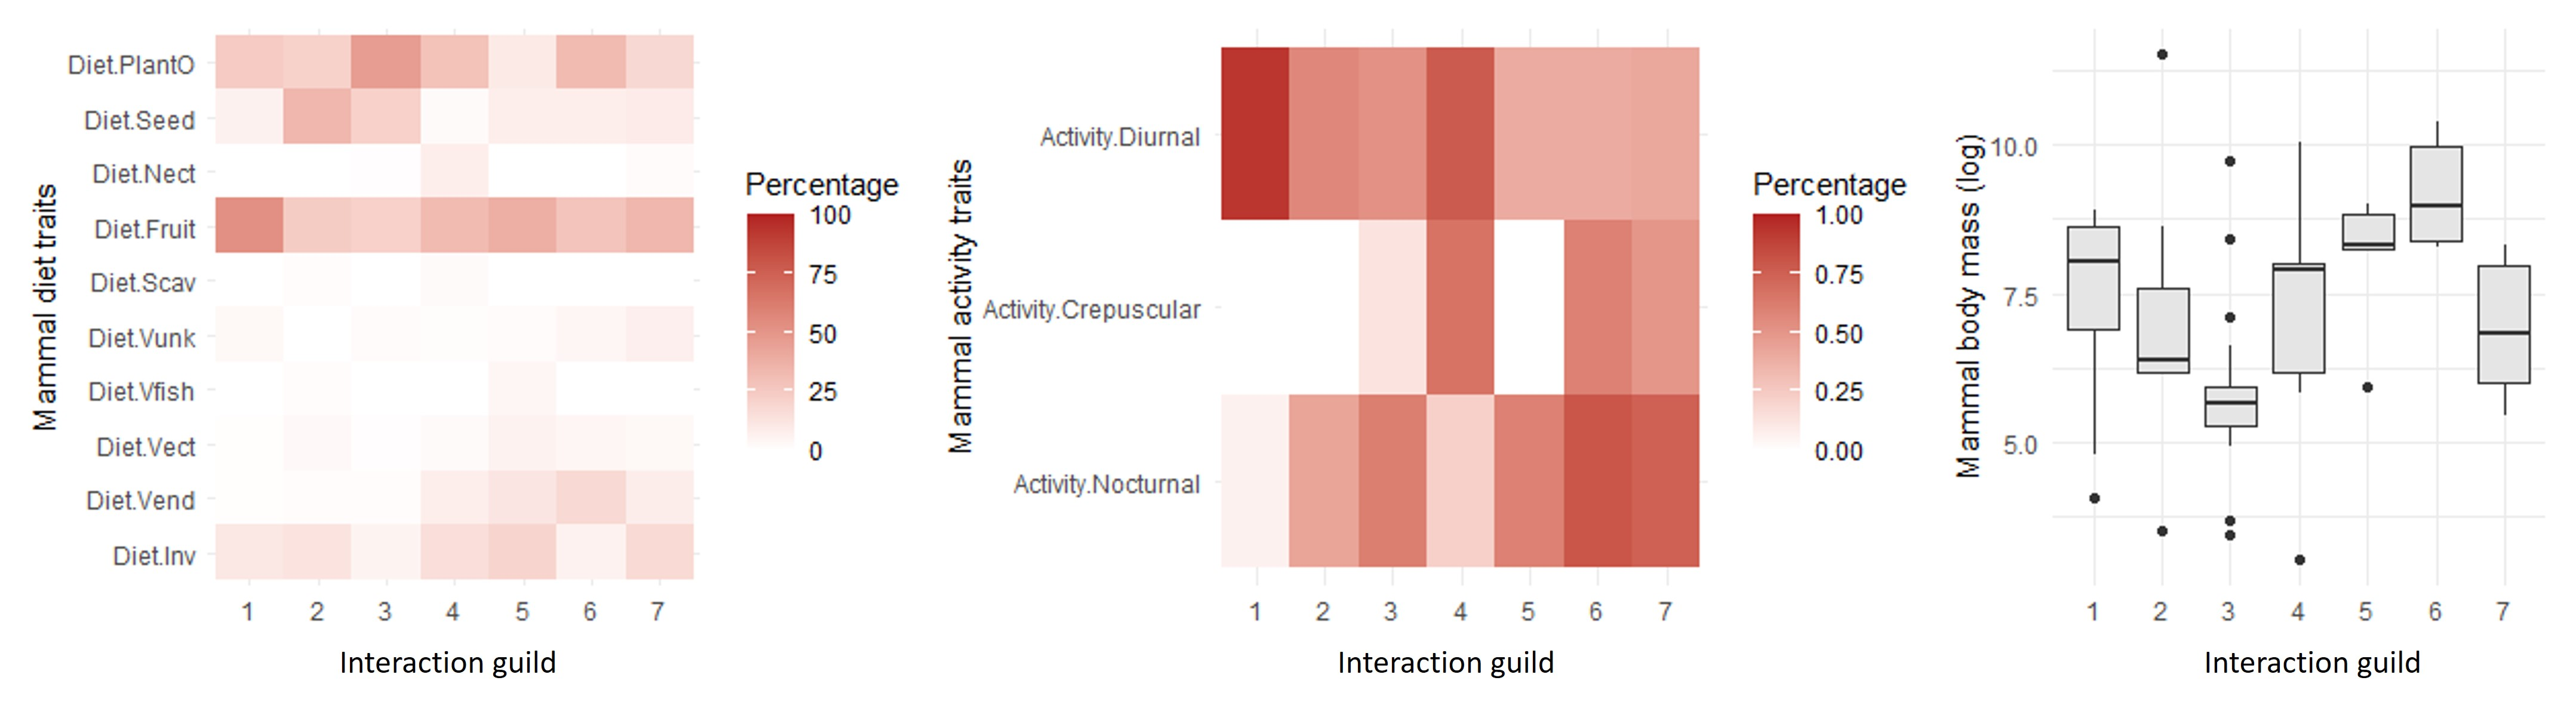
\includegraphics[width=5.67708in,height=\textheight,keepaspectratio]{sup_figures/mammal_trait_sbm.jpg}

}

\caption{Data imbalance}

\end{figure}%

\subsection{Supplementary Figure 8}

\begin{figure}[H]

{\centering 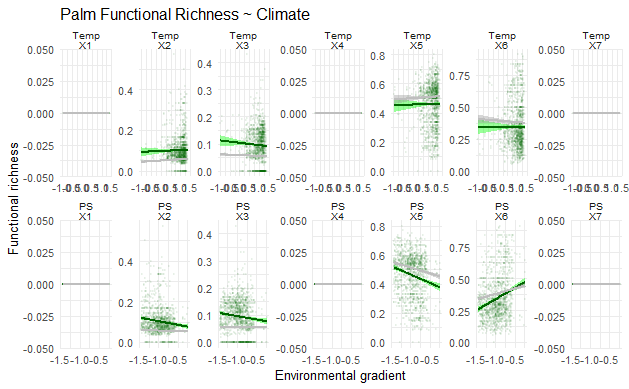
\includegraphics[width=5.67708in,height=\textheight,keepaspectratio]{sup_figures/palm_FR_detail.jpg}

}

\caption{Data imbalance}

\end{figure}%

\subsection{Supplementary Figure 9}

\begin{figure}[H]

{\centering 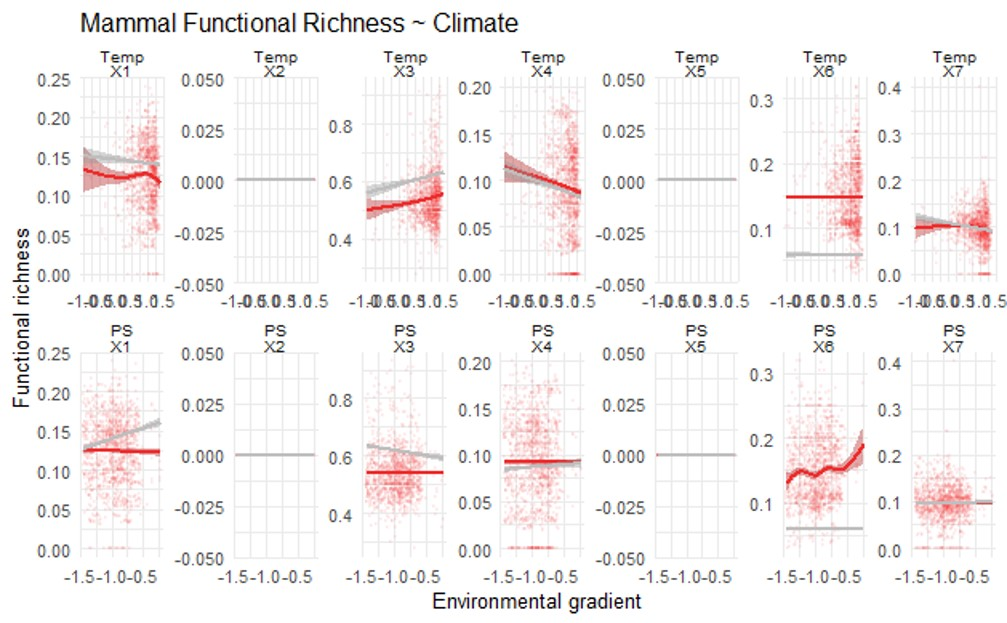
\includegraphics[width=5.67708in,height=\textheight,keepaspectratio]{sup_figures/mammal_FR_detail.jpg}

}

\caption{Data imbalance}

\end{figure}%

\subsection{Supplementary Figure 10}

\begin{figure}[H]

{\centering 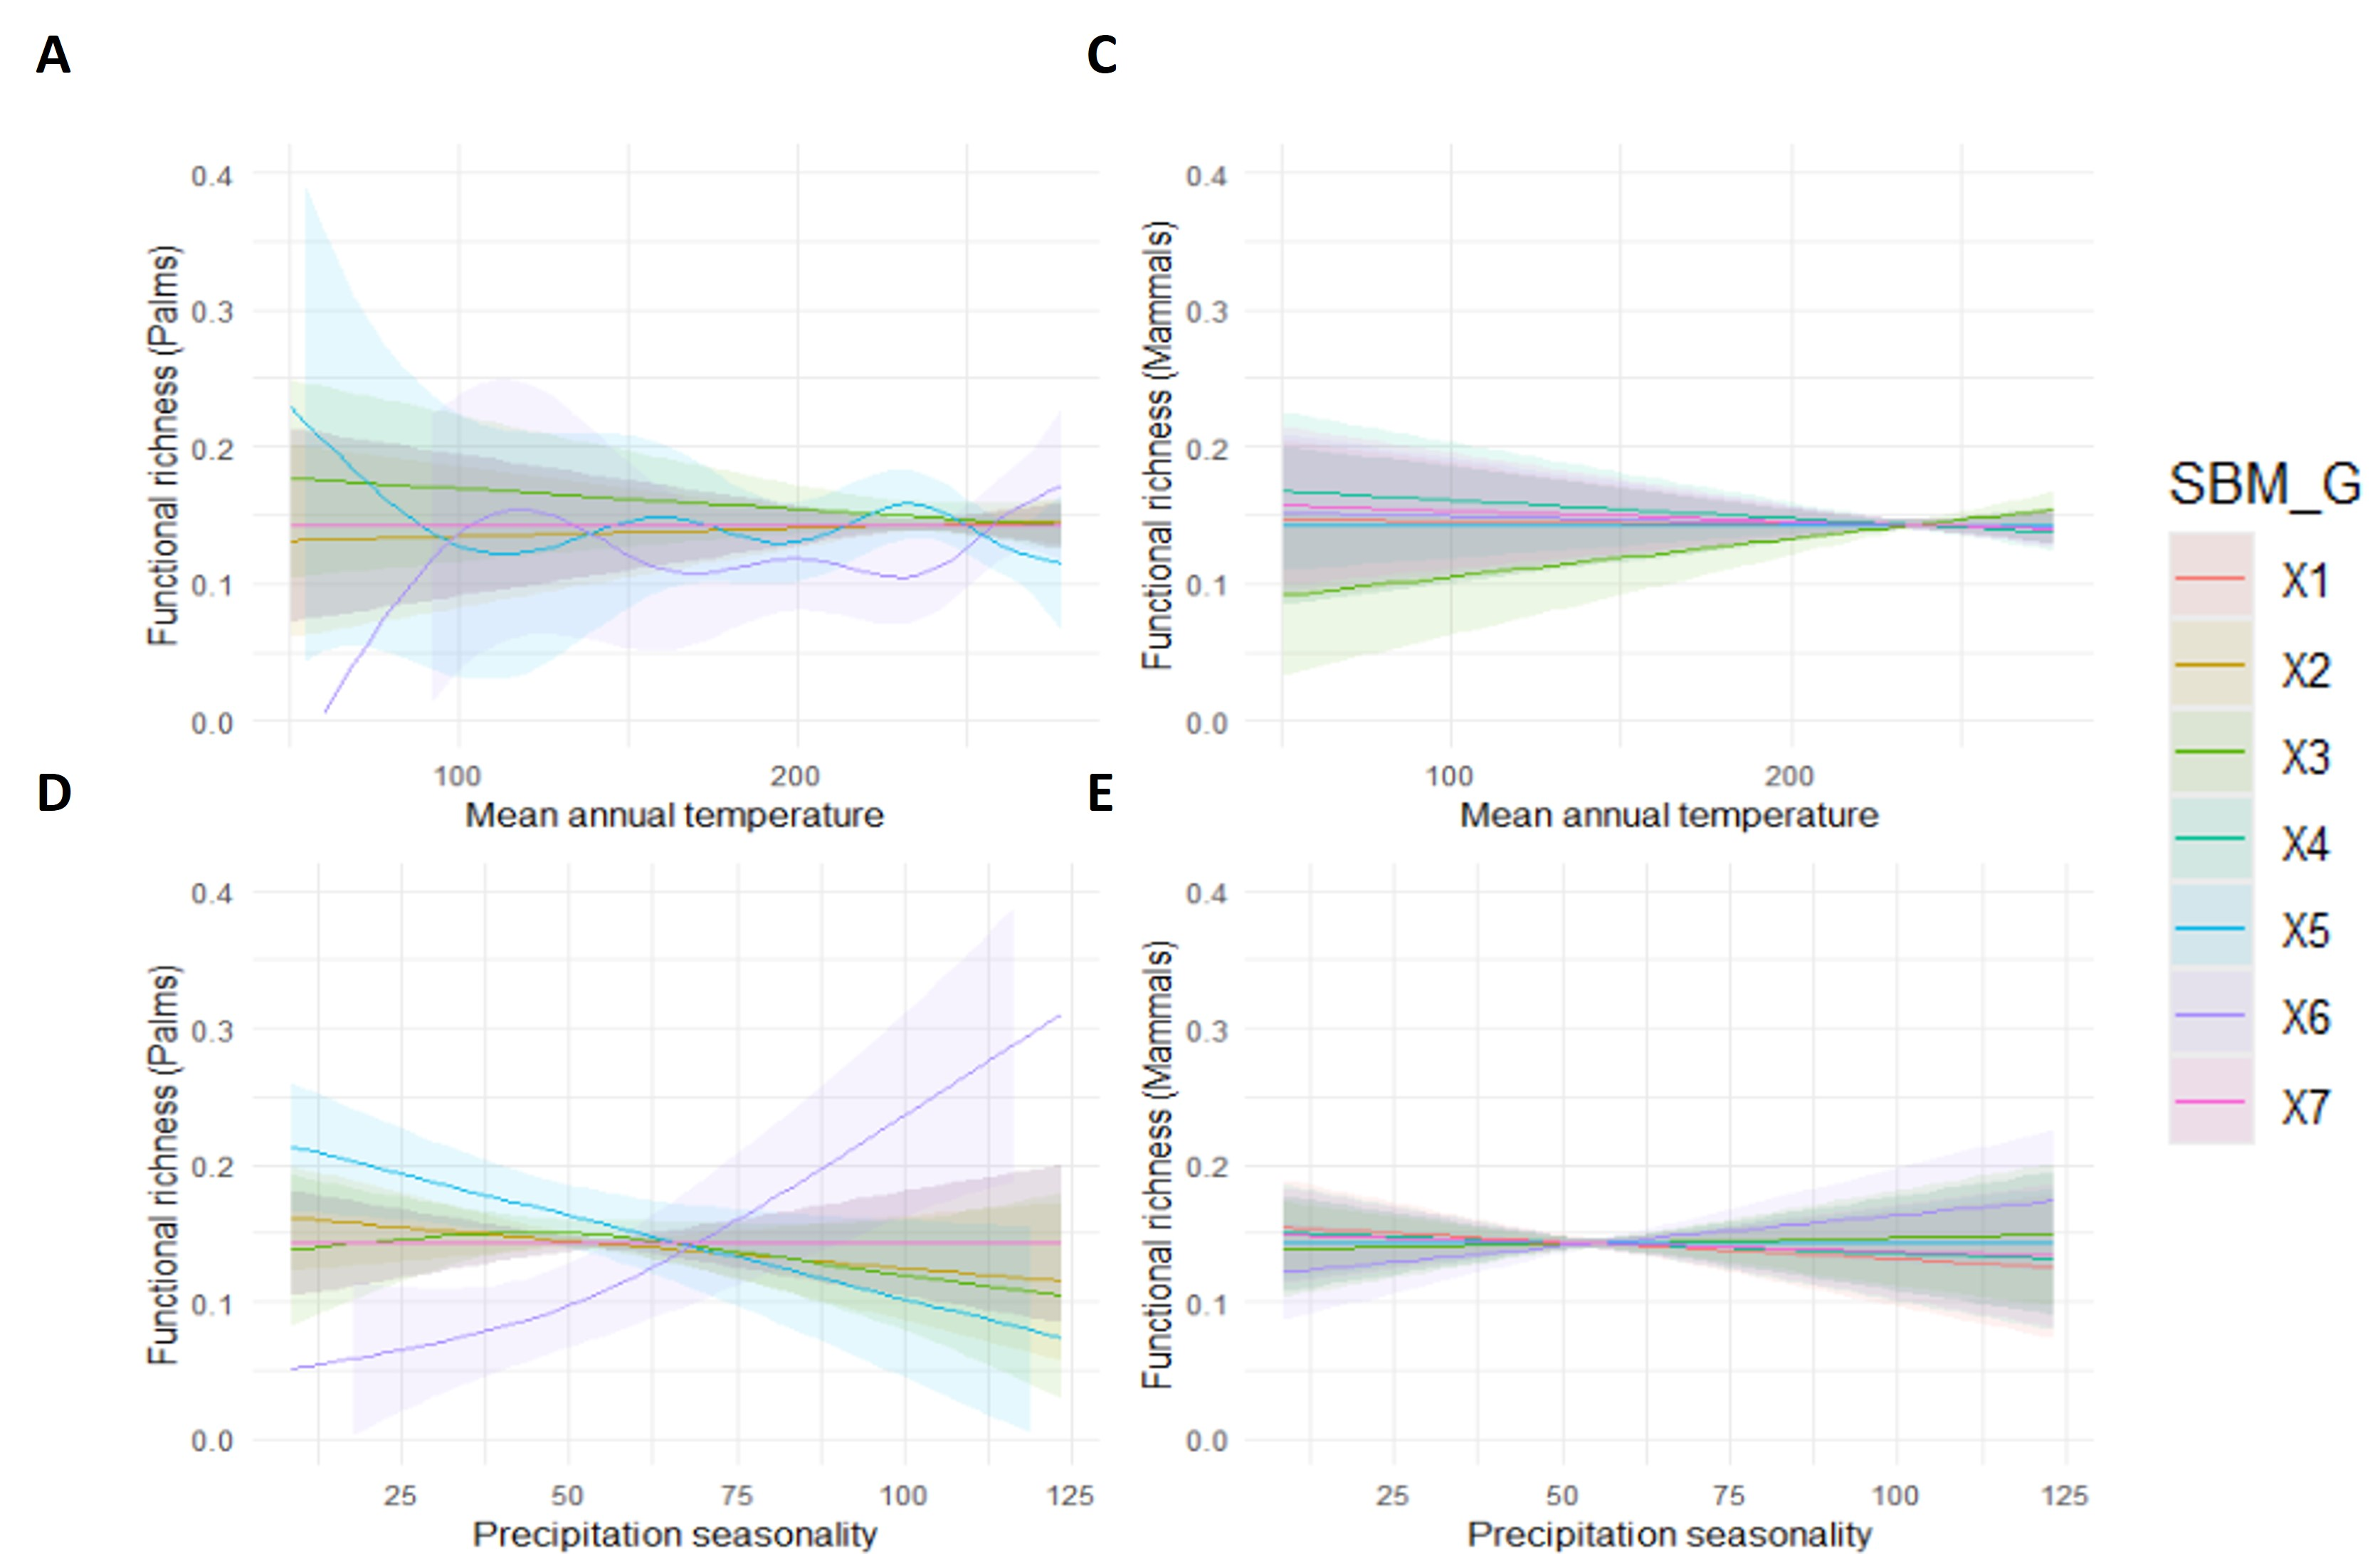
\includegraphics[width=5.67708in,height=\textheight,keepaspectratio]{sup_figures/fr_model_predictions.jpg}

}

\caption{Data imbalance}

\end{figure}%

\subsection{Supplementary Figure 11}

\begin{figure}[H]

{\centering 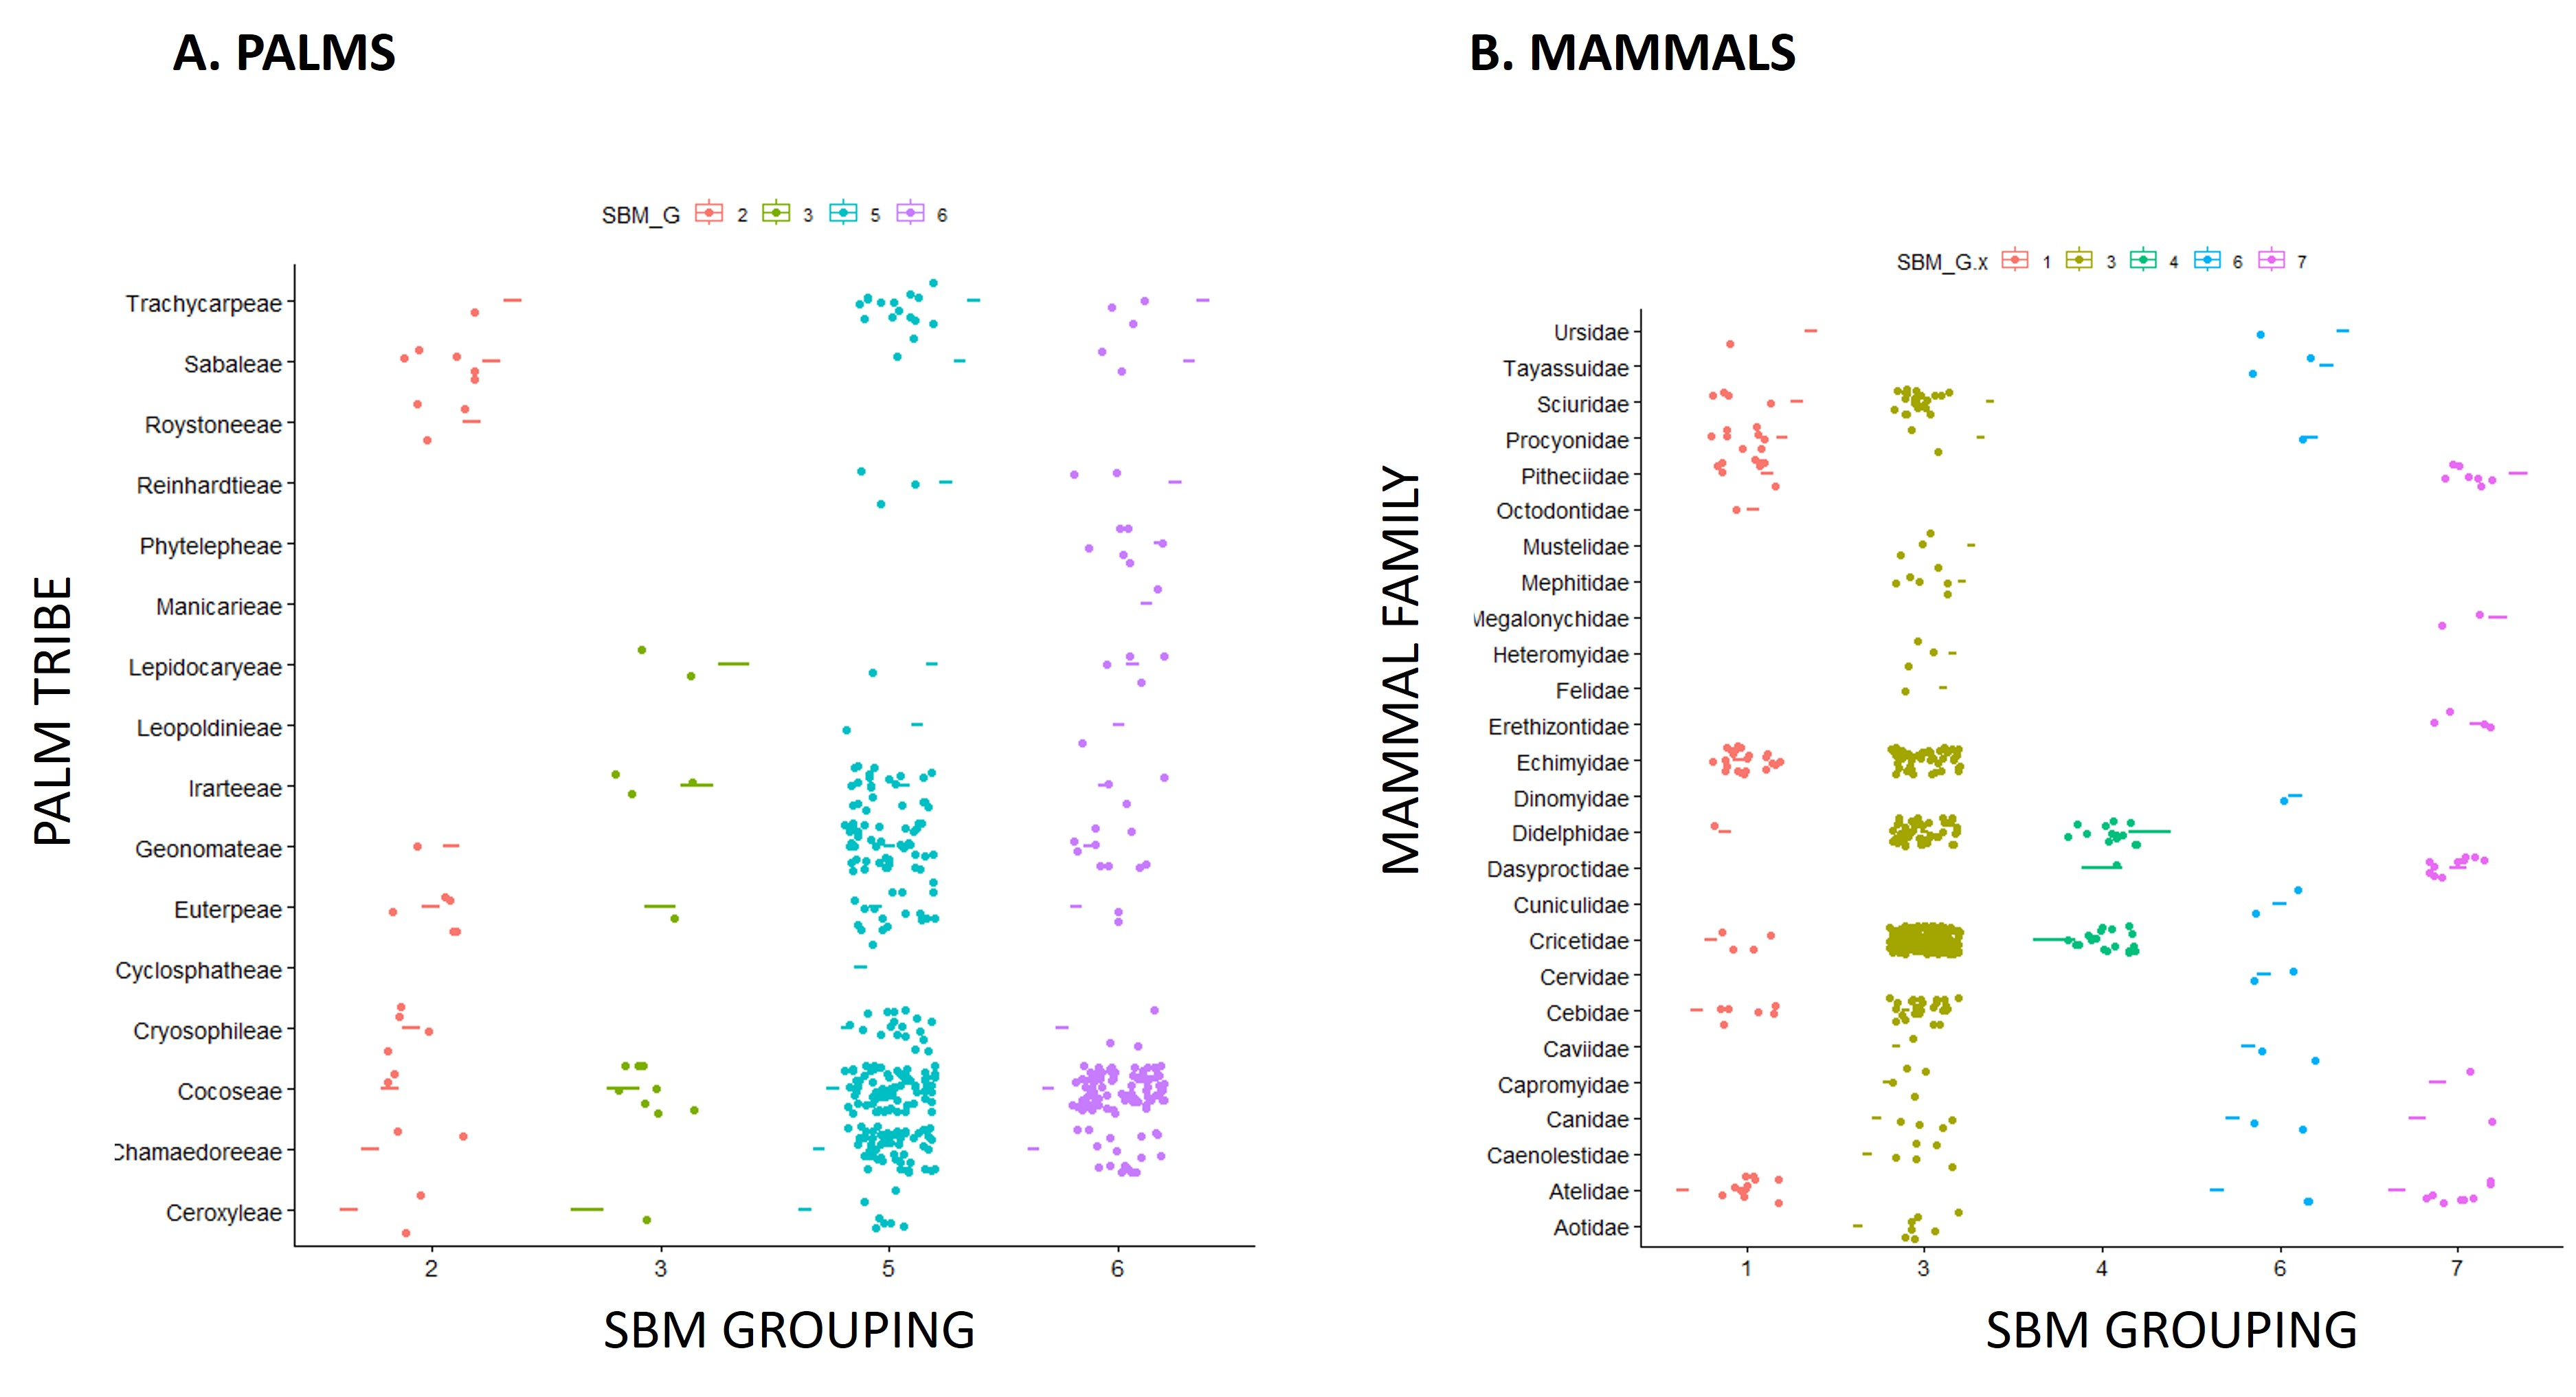
\includegraphics[width=5.67708in,height=\textheight,keepaspectratio]{sup_figures/sup_SBM_taxonomy.jpg}

}

\caption{Data imbalance}

\end{figure}%

\subsection{Supplementary Figure 12}

\begin{figure}[H]

{\centering 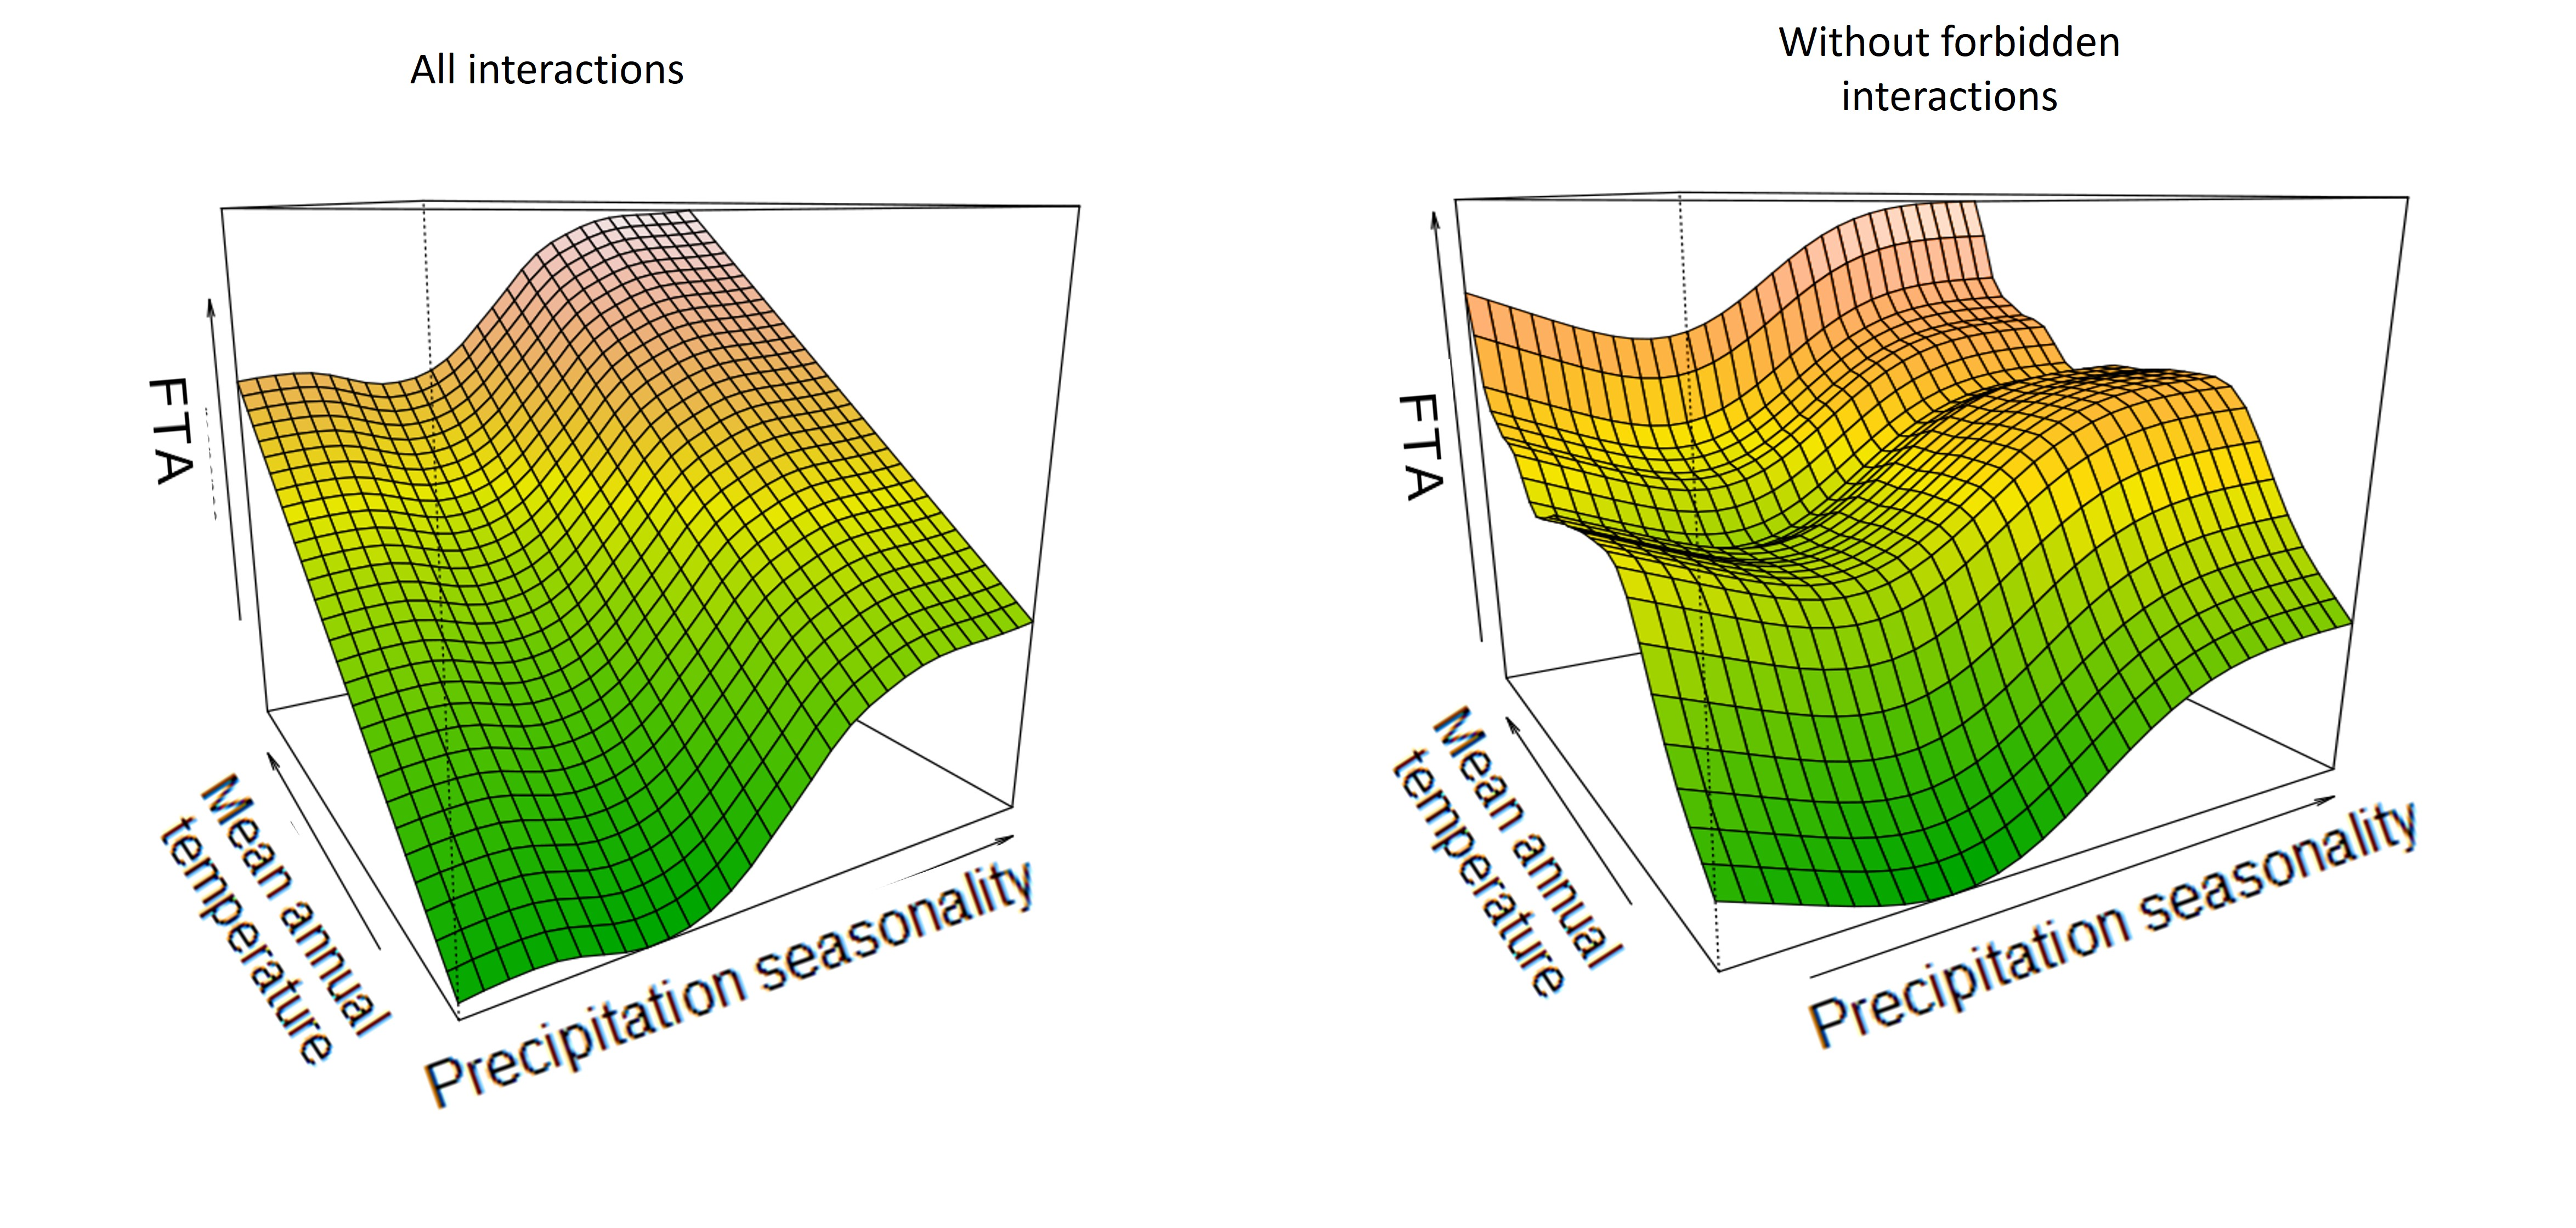
\includegraphics[width=5.67708in,height=\textheight,keepaspectratio]{sup_figures/fta_surface_both.jpg}

}

\caption{Data imbalance}

\end{figure}%

\section{Suplementary Tables}\label{suplementary-tables}

\subsubsection{Supplementary Table 1a:}\label{supplementary-table-1a}

Summary of parametric and smooth term coefficients for models predicting
ecological responses in the Functional Richness of interaction relevant
traits of Palms. The parametric coefficients include estimates, standard
errors, t-values, and p-values for each predictor (Intercept, Mean
annual temperature (Temp), Total annual precipitation (Prec),
Temperature seasonality (TS), and Precipitation seasonality (PS) ).
Smooth terms are shown for each predictor in combination with ecological
guilds (Guild\_X1 through Guild\_X7), providing the effective degrees of
freedom (edf), reference degrees of freedom (Ref.df), F-statistics, and
p-values for each interaction. Significant p-values are highlighted,
indicating where predictor-guild interactions have a statistically
significant effect on the response variable.

\begin{longtable}[]{@{}
  >{\centering\arraybackslash}p{(\linewidth - 8\tabcolsep) * \real{0.2000}}
  >{\centering\arraybackslash}p{(\linewidth - 8\tabcolsep) * \real{0.2000}}
  >{\centering\arraybackslash}p{(\linewidth - 8\tabcolsep) * \real{0.2000}}
  >{\centering\arraybackslash}p{(\linewidth - 8\tabcolsep) * \real{0.2000}}
  >{\centering\arraybackslash}p{(\linewidth - 8\tabcolsep) * \real{0.2000}}@{}}
\toprule\noalign{}
\endhead
\bottomrule\noalign{}
\endlastfoot
~ &
\multicolumn{4}{>{\centering\arraybackslash}p{(\linewidth - 8\tabcolsep) * \real{0.8000} + 6\tabcolsep}@{}}{%
Dependent variable} \\
Predictors & Estimates & std. Error & CI & p \\
(Intercept) & 0.01 & 0.01 & -0.01~--~0.03 & 0.335 \\
Temp & 0.00 & 0.00 & 0.00~--~0.00 & \textbf{0.003} \\
Prec & 0.00 & 0.00 & -0.00~--~0.00 & 0.233 \\
TS & -0.00 & 0.00 & -0.00~--~0.00 & 0.789 \\
PS & 0.00 & 0.00 & -0.00~--~0.00 & 0.499 \\
\begin{minipage}[t]{\linewidth}\raggedright
Smooth term (Temp) × SBM\\
GX1\strut
\end{minipage} & & & & 0.073 \\
\begin{minipage}[t]{\linewidth}\raggedright
Smooth term (Temp) × SBM\\
GX2\strut
\end{minipage} & & & & 0.129 \\
\begin{minipage}[t]{\linewidth}\raggedright
Smooth term (Temp) × SBM\\
GX3\strut
\end{minipage} & & & & \textbf{0.014} \\
\begin{minipage}[t]{\linewidth}\raggedright
Smooth term (Temp) × SBM\\
GX4\strut
\end{minipage} & & & & 0.073 \\
\begin{minipage}[t]{\linewidth}\raggedright
Smooth term (Temp) × SBM\\
GX5\strut
\end{minipage} & & & & 0.067 \\
\begin{minipage}[t]{\linewidth}\raggedright
Smooth term (Temp) × SBM\\
GX6\strut
\end{minipage} & & & & 0.207 \\
\begin{minipage}[t]{\linewidth}\raggedright
Smooth term (Temp) × SBM\\
GX7\strut
\end{minipage} & & & & 0.073 \\
\begin{minipage}[t]{\linewidth}\raggedright
Smooth term (Prec) × SBM\\
GX1\strut
\end{minipage} & & & & 0.331 \\
\begin{minipage}[t]{\linewidth}\raggedright
Smooth term (Prec) × SBM\\
GX2\strut
\end{minipage} & & & & 0.292 \\
\begin{minipage}[t]{\linewidth}\raggedright
Smooth term (Prec) × SBM\\
GX3\strut
\end{minipage} & & & & 0.392 \\
\begin{minipage}[t]{\linewidth}\raggedright
Smooth term (Prec) × SBM\\
GX4\strut
\end{minipage} & & & & 0.331 \\
\begin{minipage}[t]{\linewidth}\raggedright
Smooth term (Prec) × SBM\\
GX5\strut
\end{minipage} & & & & 0.637 \\
\begin{minipage}[t]{\linewidth}\raggedright
Smooth term (Prec) × SBM\\
GX6\strut
\end{minipage} & & & & \textbf{0.007} \\
\begin{minipage}[t]{\linewidth}\raggedright
Smooth term (Prec) × SBM\\
GX7\strut
\end{minipage} & & & & 0.331 \\
\begin{minipage}[t]{\linewidth}\raggedright
Smooth term (TS) × SBM\\
GX1\strut
\end{minipage} & & & & 0.864 \\
\begin{minipage}[t]{\linewidth}\raggedright
Smooth term (TS) × SBM\\
GX2\strut
\end{minipage} & & & & 0.863 \\
\begin{minipage}[t]{\linewidth}\raggedright
Smooth term (TS) × SBM\\
GX3\strut
\end{minipage} & & & & 0.868 \\
\begin{minipage}[t]{\linewidth}\raggedright
Smooth term (TS) × SBM\\
GX4\strut
\end{minipage} & & & & 0.864 \\
\begin{minipage}[t]{\linewidth}\raggedright
Smooth term (TS) × SBM\\
GX5\strut
\end{minipage} & & & & 0.890 \\
\begin{minipage}[t]{\linewidth}\raggedright
Smooth term (TS) × SBM\\
GX6\strut
\end{minipage} & & & & 0.352 \\
\begin{minipage}[t]{\linewidth}\raggedright
Smooth term (TS) × SBM\\
GX7\strut
\end{minipage} & & & & 0.864 \\
\begin{minipage}[t]{\linewidth}\raggedright
Smooth term (PS) × SBM\\
GX1\strut
\end{minipage} & & & & 0.705 \\
\begin{minipage}[t]{\linewidth}\raggedright
Smooth term (PS) × SBM\\
GX2\strut
\end{minipage} & & & & 0.199 \\
\begin{minipage}[t]{\linewidth}\raggedright
Smooth term (PS) × SBM\\
GX3\strut
\end{minipage} & & & & 0.239 \\
\begin{minipage}[t]{\linewidth}\raggedright
Smooth term (PS) × SBM\\
GX4\strut
\end{minipage} & & & & 0.705 \\
\begin{minipage}[t]{\linewidth}\raggedright
Smooth term (PS) × SBM\\
GX5\strut
\end{minipage} & & & & \textbf{0.007} \\
\begin{minipage}[t]{\linewidth}\raggedright
Smooth term (PS) × SBM\\
GX6\strut
\end{minipage} & & & & \textbf{0.001} \\
\begin{minipage}[t]{\linewidth}\raggedright
Smooth term (PS) × SBM\\
GX7\strut
\end{minipage} & & & & 0.705 \\
Observations &
\multicolumn{4}{>{\raggedright\arraybackslash}p{(\linewidth - 8\tabcolsep) * \real{0.8000} + 6\tabcolsep}@{}}{%
9009} \\
R\textsuperscript{2} &
\multicolumn{4}{>{\raggedright\arraybackslash}p{(\linewidth - 8\tabcolsep) * \real{0.8000} + 6\tabcolsep}@{}}{%
0.012} \\
\end{longtable}

\textsubscript{Source:
\href{https://lessardlab.github.io/FTA-Neotropics/index.qmd.html}{Article
Notebook}}

\subsubsection{Supplementary Table 1b:}\label{supplementary-table-1b}

Summary of parametric and smooth term coefficients for models predicting
ecological responses in the Functional Richness of interaction relevant
traits of frugivore Mammals. The parametric coefficients include
estimates, standard errors, t-values, and p-values for each predictor
(Intercept, Mean annual temperature (Temp), Total annual precipitation
(Prec), Temperature seasonality (TS), and Precipitation seasonality (PS)
). Smooth terms are shown for each predictor in combination with
ecological guilds (Guild\_X1 through Guild\_X7), providing the effective
degrees of freedom (edf), reference degrees of freedom (Ref.df),
F-statistics, and p-values for each interaction. Significant p-values
are highlighted, indicating where predictor-guild interactions have a
statistically significant effect on the response variable.

\begin{longtable}[]{@{}
  >{\centering\arraybackslash}p{(\linewidth - 8\tabcolsep) * \real{0.2000}}
  >{\centering\arraybackslash}p{(\linewidth - 8\tabcolsep) * \real{0.2000}}
  >{\centering\arraybackslash}p{(\linewidth - 8\tabcolsep) * \real{0.2000}}
  >{\centering\arraybackslash}p{(\linewidth - 8\tabcolsep) * \real{0.2000}}
  >{\centering\arraybackslash}p{(\linewidth - 8\tabcolsep) * \real{0.2000}}@{}}
\toprule\noalign{}
\endhead
\bottomrule\noalign{}
\endlastfoot
~ &
\multicolumn{4}{>{\centering\arraybackslash}p{(\linewidth - 8\tabcolsep) * \real{0.8000} + 6\tabcolsep}@{}}{%
Dependent variable} \\
Predictors & Estimates & std. Error & CI & p \\
(Intercept) & 0.01 & 0.00 & 0.01~--~0.02 & \textbf{\textless0.001} \\
Temp & 0.00 & 0.00 & 0.00~--~0.00 & \textbf{\textless0.001} \\
Prec & 0.00 & 0.00 & -0.00~--~0.00 & 0.153 \\
TS & 0.00 & 0.00 & -0.00~--~0.00 & 0.633 \\
PS & 0.00 & 0.00 & -0.00~--~0.00 & 0.128 \\
\begin{minipage}[t]{\linewidth}\raggedright
Smooth term (Temp) × SBM\\
GX1\strut
\end{minipage} & & & & \textbf{0.011} \\
\begin{minipage}[t]{\linewidth}\raggedright
Smooth term (Temp) × SBM\\
GX2\strut
\end{minipage} & & & & \textbf{0.010} \\
\begin{minipage}[t]{\linewidth}\raggedright
Smooth term (Temp) × SBM\\
GX3\strut
\end{minipage} & & & & 0.331 \\
\begin{minipage}[t]{\linewidth}\raggedright
Smooth term (Temp) × SBM\\
GX4\strut
\end{minipage} & & & & \textbf{0.001} \\
\begin{minipage}[t]{\linewidth}\raggedright
Smooth term (Temp) × SBM\\
GX5\strut
\end{minipage} & & & & \textbf{0.010} \\
\begin{minipage}[t]{\linewidth}\raggedright
Smooth term (Temp) × SBM\\
GX6\strut
\end{minipage} & & & & \textbf{0.002} \\
\begin{minipage}[t]{\linewidth}\raggedright
Smooth term (Temp) × SBM\\
GX7\strut
\end{minipage} & & & & \textbf{0.003} \\
\begin{minipage}[t]{\linewidth}\raggedright
Smooth term (Prec) × SBM\\
GX1\strut
\end{minipage} & & & & 0.322 \\
\begin{minipage}[t]{\linewidth}\raggedright
Smooth term (Prec) × SBM\\
GX2\strut
\end{minipage} & & & & 0.541 \\
\begin{minipage}[t]{\linewidth}\raggedright
Smooth term (Prec) × SBM\\
GX3\strut
\end{minipage} & & & & 0.552 \\
\begin{minipage}[t]{\linewidth}\raggedright
Smooth term (Prec) × SBM\\
GX4\strut
\end{minipage} & & & & 0.449 \\
\begin{minipage}[t]{\linewidth}\raggedright
Smooth term (Prec) × SBM\\
GX5\strut
\end{minipage} & & & & 0.541 \\
\begin{minipage}[t]{\linewidth}\raggedright
Smooth term (Prec) × SBM\\
GX6\strut
\end{minipage} & & & & 0.950 \\
\begin{minipage}[t]{\linewidth}\raggedright
Smooth term (Prec) × SBM\\
GX7\strut
\end{minipage} & & & & 0.436 \\
\begin{minipage}[t]{\linewidth}\raggedright
Smooth term (TS) × SBM\\
GX1\strut
\end{minipage} & & & & 0.654 \\
\begin{minipage}[t]{\linewidth}\raggedright
Smooth term (TS) × SBM\\
GX2\strut
\end{minipage} & & & & 0.849 \\
\begin{minipage}[t]{\linewidth}\raggedright
Smooth term (TS) × SBM\\
GX3\strut
\end{minipage} & & & & 0.748 \\
\begin{minipage}[t]{\linewidth}\raggedright
Smooth term (TS) × SBM\\
GX4\strut
\end{minipage} & & & & 0.678 \\
\begin{minipage}[t]{\linewidth}\raggedright
Smooth term (TS) × SBM\\
GX5\strut
\end{minipage} & & & & 0.849 \\
\begin{minipage}[t]{\linewidth}\raggedright
Smooth term (TS) × SBM\\
GX6\strut
\end{minipage} & & & & 0.920 \\
\begin{minipage}[t]{\linewidth}\raggedright
Smooth term (TS) × SBM\\
GX7\strut
\end{minipage} & & & & 0.611 \\
\begin{minipage}[t]{\linewidth}\raggedright
Smooth term (PS) × SBM\\
GX1\strut
\end{minipage} & & & & 0.225 \\
\begin{minipage}[t]{\linewidth}\raggedright
Smooth term (PS) × SBM\\
GX2\strut
\end{minipage} & & & & 0.568 \\
\begin{minipage}[t]{\linewidth}\raggedright
Smooth term (PS) × SBM\\
GX3\strut
\end{minipage} & & & & 0.748 \\
\begin{minipage}[t]{\linewidth}\raggedright
Smooth term (PS) × SBM\\
GX4\strut
\end{minipage} & & & & 0.314 \\
\begin{minipage}[t]{\linewidth}\raggedright
Smooth term (PS) × SBM\\
GX5\strut
\end{minipage} & & & & 0.568 \\
\begin{minipage}[t]{\linewidth}\raggedright
Smooth term (PS) × SBM\\
GX6\strut
\end{minipage} & & & & 0.549 \\
\begin{minipage}[t]{\linewidth}\raggedright
Smooth term (PS) × SBM\\
GX7\strut
\end{minipage} & & & & 0.361 \\
Observations &
\multicolumn{4}{>{\raggedright\arraybackslash}p{(\linewidth - 8\tabcolsep) * \real{0.8000} + 6\tabcolsep}@{}}{%
9009} \\
R\textsuperscript{2} &
\multicolumn{4}{>{\raggedright\arraybackslash}p{(\linewidth - 8\tabcolsep) * \real{0.8000} + 6\tabcolsep}@{}}{%
-0.002} \\
\end{longtable}

\textsubscript{Source:
\href{https://lessardlab.github.io/FTA-Neotropics/index.qmd.html}{Article
Notebook}}

\phantomsection\label{refs}
\begin{CSLReferences}{1}{0}
\bibitem[\citeproctext]{ref-acevedo2020sampling}
Acevedo-Quintero, J. F., Saldaña-Vázquez, R. A., Mendoza, E., \&
Zamora-Abrego, J. G. (2020). Sampling bias affects the relationship
between structural importance and species body mass in frugivore-plant
interaction networks. \emph{Ecological Complexity}, \emph{44}, 100870.

\bibitem[\citeproctext]{ref-ackerly2003community}
Ackerly, D. D. (2003). Community assembly, niche conservatism, and
adaptive evolution in changing environments. \emph{International Journal
of Plant Sciences}, \emph{164}(S3), S165--S184.

\bibitem[\citeproctext]{ref-albrecht2018plant}
Albrecht, J., Classen, A., Vollstädt, M. G., Mayr, A., Mollel, N. P.,
Schellenberger Costa, D., et al. (2018). Plant and animal functional
diversity drive mutualistic network assembly across an elevational
gradient. \emph{Nature Communications}, \emph{9}(1), 3177.

\bibitem[\citeproctext]{ref-allesina2008general}
Allesina, S., Alonso, D., \& Pascual, M. (2008). A general model for
food web structure. \emph{Science}, \emph{320}(5876), 658--661.

\bibitem[\citeproctext]{ref-bello2023analyzing}
Bello, C., Schleuning, M., \& Graham, C. H. (2023). Analyzing trophic
ecosystem functions with the interaction functional space. \emph{Trends
in Ecology \& Evolution}.

\bibitem[\citeproctext]{ref-bluthgen2011functional}
Blüthgen, N., \& Klein, A.-M. (2011). Functional complementarity and
specialisation: The role of biodiversity in plant--pollinator
interactions. \emph{Basic and Applied Ecology}, \emph{12}(4), 282--291.

\bibitem[\citeproctext]{ref-bluthgen2006measuring}
Blüthgen, N., Menzel, F., \& Blüthgen, N. (2006). Measuring
specialization in species interaction networks. \emph{BMC Ecology},
\emph{6}(1), 1--12.

\bibitem[\citeproctext]{ref-bluthgen2007specialization}
Blüthgen, N., Menzel, F., Hovestadt, T., Fiala, B., \& Blüthgen, N.
(2007). Specialization, constraints, and conflicting interests in
mutualistic networks. \emph{Current Biology}, \emph{17}(4), 341--346.

\bibitem[\citeproctext]{ref-bogoni2020extent}
Bogoni, J. A., Peres, C. A., \& Ferraz, K. M. (2020). Extent, intensity
and drivers of mammal defaunation: A continental-scale analysis across
the neotropics. \emph{Scientific Reports}, \emph{10}(1), 14750.

\bibitem[\citeproctext]{ref-dehling2018structure}
Dehling, D. M. (2018). The structure of ecological networks.
\emph{Ecological Networks in the Tropics: An Integrative Overview of
Species Interactions From Some of the Most Species-Rich Habitats on
Earth}, 29--42.

\bibitem[\citeproctext]{ref-dehling2014functional}
Dehling, D. M., Töpfer, T., Schaefer, H. M., Jordano, P., Böhning-Gaese,
K., \& Schleuning, M. (2014). Functional relationships beyond species
richness patterns: Trait matching in plant--bird mutualisms across
scales. \emph{Global Ecology and Biogeography}, \emph{23}(10),
1085--1093.

\bibitem[\citeproctext]{ref-dehling2020similar}
Dehling, D. M., Peralta, G., Bender, I. M., Blendinger, P. G.,
Böhning-Gaese, K., Muñoz, M. C., et al. (2020). Similar composition of
functional roles in andean seed-dispersal networks, despite high species
and interaction turnover. \emph{Ecology}, \emph{101}(7), e03028.

\bibitem[\citeproctext]{ref-donoso2017complementary}
Donoso, I., Garcı́a, D., Martı́nez, D., Tylianakis, J. M., \& Stouffer, D.
B. (2017). Complementary effects of species abundances and ecological
neighborhood on the occurrence of fruit-frugivore interactions.
\emph{Frontiers in Ecology and Evolution}, 133.

\bibitem[\citeproctext]{ref-donoso2020downsizing}
Donoso, I., Sorensen, M. C., Blendinger, P. G., Kissling, W. D.,
Neuschulz, E. L., Mueller, T., \& Schleuning, M. (2020). Downsizing of
animal communities triggers stronger functional than structural decay in
seed-dispersal networks. \emph{Nature Communications}, \emph{11}(1),
1582.

\bibitem[\citeproctext]{ref-emer2020seed}
Emer, C., Jordano, P., Pizo, M. A., Ribeiro, M. C., Silva, F. R. da, \&
Galetti, M. (2020). Seed dispersal networks in tropical forest
fragments: Area effects, remnant species, and interaction diversity.
\emph{Biotropica}, \emph{52}(1), 81--89.

\bibitem[\citeproctext]{ref-garcia2018frugivore}
Garcı́a, D., Donoso, I., \& Rodrı́guez-Pérez, J. (2018). Frugivore
biodiversity and complementarity in interaction networks enhance
landscape-scale seed dispersal function. \emph{Functional Ecology},
\emph{32}(12), 2742--2752.

\bibitem[\citeproctext]{ref-guzman2019towards}
Guzman, L. M., Germain, R. M., Forbes, C., Straus, S., O'Connor, M. I.,
Gravel, D., et al. (2019). Towards a multi-trophic extension of
metacommunity ecology. \emph{Ecology Letters}, \emph{22}(1), 19--33.

\bibitem[\citeproctext]{ref-halpern2008functional}
Halpern, B. S., \& Floeter, S. R. (2008). Functional diversity responses
to changing species richness in reef fish communities. \emph{Marine
Ecology Progress Series}, \emph{364}, 147--156.

\bibitem[\citeproctext]{ref-hillerislambers2012rethinking}
HilleRisLambers, J., Adler, P. B., Harpole, W. S., Levine, J. M., \&
Mayfield, M. M. (2012). Rethinking community assembly through the lens
of coexistence theory. \emph{Annual Review of Ecology, Evolution, and
Systematics}, \emph{43}, 227--248.

\bibitem[\citeproctext]{ref-hoekstra2001mechanisms}
Hoekstra, F. A., Golovina, E. A., \& Buitink, J. (2001). Mechanisms of
plant desiccation tolerance. \emph{Trends in Plant Science},
\emph{6}(9), 431--438.

\bibitem[\citeproctext]{ref-kraft2010functional}
Kraft, N. J., \& Ackerly, D. D. (2010). Functional trait and
phylogenetic tests of community assembly across spatial scales in an
amazonian forest. \emph{Ecological Monographs}, \emph{80}(3), 401--422.

\bibitem[\citeproctext]{ref-kraft2008functional}
Kraft, N. J., Valencia, R., \& Ackerly, D. D. (2008). Functional traits
and niche-based tree community assembly in an amazonian forest.
\emph{Science}, \emph{322}(5901), 580--582.

\bibitem[\citeproctext]{ref-kraft2015community}
Kraft, N. J., Adler, P. B., Godoy, O., James, E. C., Fuller, S., \&
Levine, J. M. (2015). Community assembly, coexistence and the
environmental filtering metaphor. \emph{Functional Ecology},
\emph{29}(5), 592--599.

\bibitem[\citeproctext]{ref-laliberte2010distance}
Laliberté, E., \& Legendre, P. (2010). A distance-based framework for
measuring functional diversity from multiple traits. \emph{Ecology},
\emph{91}(1), 299--305.

\bibitem[\citeproctext]{ref-lavorel2013novel}
Lavorel, S., Storkey, J., Bardgett, R. D., De Bello, F., Berg, M. P., Le
Roux, X., et al. (2013). A novel framework for linking functional
diversity of plants with other trophic levels for the quantification of
ecosystem services. \emph{Journal of Vegetation Science}, \emph{24}(5),
942--948.

\bibitem[\citeproctext]{ref-marjakangas2022trait}
Marjakangas, E.-L., Muñoz, G., Turney, S., Albrecht, J., Neuschulz, E.
L., Schleuning, M., \& Lessard, J.-P. (2022). Trait-based inference of
ecological network assembly: A conceptual framework and methodological
toolbox. \emph{Ecological Monographs}, \emph{92}(2), e1502.

\bibitem[\citeproctext]{ref-marques2022mutualism}
Marques Dracxler, C., \& Kissling, W. D. (2022). The
mutualism--antagonism continuum in neotropical palm--frugivore
interactions: From interaction outcomes to ecosystem dynamics.
\emph{Biological Reviews}, \emph{97}(2), 527--553.

\bibitem[\citeproctext]{ref-mccain2014body}
McCain, C. M., \& King, S. R. (2014). Body size and activity times
mediate mammalian responses to climate change. \emph{Global Change
Biology}, \emph{20}(6), 1760--1769.

\bibitem[\citeproctext]{ref-messeder2020searching}
Messeder, J. V. S., Guerra, T. J., Dáttilo, W., \& Silveira, F. A.
(2020). Searching for keystone plant resources in fruit-frugivore
interaction networks across the neotropics. \emph{Biotropica},
\emph{52}(5), 857--870.

\bibitem[\citeproctext]{ref-moretti2009combining}
Moretti, M., \& Legg, C. (2009). Combining plant and animal traits to
assess community functional responses to disturbance. \emph{Ecography},
\emph{32}(2), 299--309.

\bibitem[\citeproctext]{ref-nagy2018arthropod}
Nagy, D. D., Magura, T., Horváth, R., Debnár, Z., \& Tóthmérész, B.
(2018). Arthropod assemblages and functional responses along an
urbanization gradient: A trait-based multi-taxa approach. \emph{Urban
Forestry \& Urban Greening}, \emph{30}, 157--168.

\bibitem[\citeproctext]{ref-paine2011functional}
Paine, C. T., Baraloto, C., Chave, J., \& Hérault, B. (2011). Functional
traits of individual trees reveal ecological constraints on community
assembly in tropical rain forests. \emph{Oikos}, \emph{120}(5),
720--727.

\bibitem[\citeproctext]{ref-pereira2022priority}
Pereira, J., Battiston, F., \& Jordán, F. (2022). Priority areas for
protection of plant-pollinator interaction networks in the atlantic
forest. \emph{Ecological Indicators}, \emph{136}, 108598.

\bibitem[\citeproctext]{ref-rohr2010modeling}
Rohr, R. P., Scherer, H., Kehrli, P., Mazza, C., \& Bersier, L.-F.
(2010). Modeling food webs: Exploring unexplained structure using latent
traits. \emph{The American Naturalist}, \emph{176}(2), 170--177.

\bibitem[\citeproctext]{ref-saravia2022ecological}
Saravia, L. A., Marina, T. I., Kristensen, N. P., De Troch, M., \& Momo,
F. R. (2022). Ecological network assembly: How the regional metaweb
influences local food webs. \emph{Journal of Animal Ecology},
\emph{91}(3), 630--642.

\bibitem[\citeproctext]{ref-schleuning2012specialization}
Schleuning, M., Fründ, J., Klein, A.-M., Abrahamczyk, S., Alarcón, R.,
Albrecht, M., et al. (2012). Specialization of mutualistic interaction
networks decreases toward tropical latitudes. \emph{Current Biology},
\emph{22}(20), 1925--1931.

\bibitem[\citeproctext]{ref-schleuning2014ecological}
Schleuning, M., Ingmann, L., Strauss, R., Fritz, S. A., Dalsgaard, B.,
Matthias Dehling, D., et al. (2014). Ecological, historical and
evolutionary determinants of modularity in weighted seed-dispersal
networks. \emph{Ecology Letters}, \emph{17}(4), 454--463.

\bibitem[\citeproctext]{ref-schleuning2020trait}
Schleuning, M., Neuschulz, E. L., Albrecht, J., Bender, I. M., Bowler,
D. E., Dehling, D. M., et al. (2020). Trait-based assessments of
climate-change impacts on interacting species. \emph{Trends in Ecology
\& Evolution}, \emph{35}(4), 319--328.

\bibitem[\citeproctext]{ref-schleuning2023animal}
Schleuning, M., Garcı́a, D., \& Tobias, J. A. (2023). Animal functional
traits: Towards a trait-based ecology for whole ecosystems.
\emph{Functional Ecology}. Wiley Online Library.

\bibitem[\citeproctext]{ref-seibold2018necessity}
Seibold, S., Cadotte, M. W., MacIvor, J. S., Thorn, S., \& Müller, J.
(2018). The necessity of multitrophic approaches in community ecology.
\emph{Trends in Ecology \& Evolution}, \emph{33}(10), 754--764.

\bibitem[\citeproctext]{ref-strydom2022food}
Strydom, T., Bouskila, S., Banville, F., Barros, C., Caron, D., Farrell,
M. J., et al. (2022). Food web reconstruction through phylogenetic
transfer of low-rank network representation. \emph{Methods in Ecology
and Evolution}, \emph{13}(12), 2838--2849.

\bibitem[\citeproctext]{ref-villeger2008new}
Villéger, S., Mason, N. W., \& Mouillot, D. (2008). New multidimensional
functional diversity indices for a multifaceted framework in functional
ecology. \emph{Ecology}, \emph{89}(8), 2290--2301.

\end{CSLReferences}




\end{document}
